\documentclass[11pt,a4paper]{article}
\usepackage[T1]{fontenc}
\usepackage[left=2cm, right=2cm, top=2cm, bottom=2cm]{geometry}
\usepackage{graphicx}
\usepackage{mathtools}
\usepackage{amssymb}
\usepackage{amsthm}
\usepackage{amsmath}

\usepackage{thmtools}
\usepackage{xcolor}
\usepackage{nameref}
\usepackage[colorlinks=true, linkcolor=blue, citecolor=cyan]{hyperref}
\usepackage{natbib} 
\usepackage{tkz-graph}
\usepackage{placeins}

\usepackage{tikz}
\usepackage{xparse}




\newcommand{\grad}{\operatorname{grad}}
\newcommand{\curl}{\operatorname{curl}}
\renewcommand{\div}{\operatorname{div}}
\newcommand{\img}{\operatorname{img}}
\renewcommand{\span}{\operatorname{span}}
\newcommand{\Z}{\mathbb{Z}}
\newcommand{\tile}[1]{\fbox{\ensuremath{#1}}}



\theoremstyle{definition}
\newtheorem{definition}{Definition}


\theoremstyle{remark}
\newtheorem{remark}{Remark}

\title{Some topological insights to the tiling problem on $ \Z^d $}
\author{Ali Fele Paranj}


\theoremstyle{definition}
\newtheorem{theorem}{Theorem}
\newtheorem{observation}{Observation}


\begin{document}
	
	\maketitle
	\begin{abstract}
		In this document I will translates some of the problems in tiling self-assembly to the language of analysis and topology, hoping to open some possible ways for using ergodic theory and other interesting analytical tools. 
	\end{abstract}
	
	
	\section{Introduction}
	
	Let's consider the set of all 2D tiles over the final alphabet $\Sigma$. The set of all such possible tilings is 
	$$ \Sigma^{\mathbb{Z}^2}, $$
	which is the same as the set of all functions from $\mathbb{Z}^2$ to $\Sigma$. 
	
	First, observe that since the alphabet is finite, assuming that it has $N$ elements, then one can write $[n] = \{1,2,3,\cdots,n\}$ in place of $\Sigma$. As far as the set structure of $\Sigma$ is considered, it is fine to do so. However, seeing these two spaces as topological spaces, one automatically assumes a discrete topology over the set $\Sigma$, however, in the case of $[n]$ one automatically assumes that 2 is "close" to 1 and 3 and far from $n$. So we might exploit this topological property of the alphabet set in deciding which tilling is plausible and which is not: based on their gluing structure, that a tile of certain type is willing to be close to the tiles of other type. Then one can possibly encode the plausible tiles as functions that are continuous given the topology of their domain $\mathbb{Z}^2$ and their range $\Sigma$. For more about the intuition behind the method see my notes in this \href{https://github.com/alifele/Lecture-Notes/blob/main/Scientific%20Notes/Some%20Intuitions%20on%20Continuous%20Maps/GraphHomologyAndCohomology.pdf}{link}.
	
	
	\section{Simple Setup}
	Define the $ d_1 $ metric on $ \Z^2 $, where
	\[ d_1\left( (n_1,n_2), (m_1,m_2) \right) = |n_1-n_2| + |m_1-m_2|. \]
	This will induce the topology where the smallest open balls are the Moor neighborhoods (see the first chapter of my \href{https://open.library.ubc.ca/soa/cIRcle/collections/ubctheses/24/items/1.0449873}{thesis} for more on this.) Also assume that we have three types of tiles $ \{ \tile{A}, \tile{B}, \tile{C} \}. $ Assuming that every tile can sit with itself (this can be relaxed later by constructing large enough product space), then the notion of ``certain tiles want to it close to certain other tiles'' will induce a partition on the set of tiles (because it is a equivalence relation). Consider the topology whose sub-basis is this partition of the set. The following figure demonstrates this partition.
	
	\begin{figure}[h!]
	\centering
	
	
	\tikzset{every picture/.style={line width=0.75pt}} %set default line width to 0.75pt        
	
	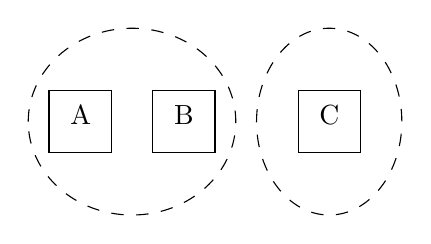
\begin{tikzpicture}[x=0.75pt,y=0.75pt,yscale=-1,xscale=1]
		%uncomment if require: \path (0,300); %set diagram left start at 0, and has height of 300
		
		%Shape: Square [id:dp45846669475066437] 
		\draw   (180,80) -- (210,80) -- (210,110) -- (180,110) -- cycle ;
		%Shape: Square [id:dp8694832240743474] 
		\draw   (230,80) -- (260,80) -- (260,110) -- (230,110) -- cycle ;
		%Shape: Square [id:dp9643149276555201] 
		\draw   (300,80) -- (330,80) -- (330,110) -- (300,110) -- cycle ;
		%Shape: Ellipse [id:dp7472268647554123] 
		\draw  [dash pattern={on 4.5pt off 4.5pt}] (170,95) .. controls (170,70.15) and (192.39,50) .. (220,50) .. controls (247.61,50) and (270,70.15) .. (270,95) .. controls (270,119.85) and (247.61,140) .. (220,140) .. controls (192.39,140) and (170,119.85) .. (170,95) -- cycle ;
		%Shape: Ellipse [id:dp9372300796607134] 
		\draw  [dash pattern={on 4.5pt off 4.5pt}] (280,95) .. controls (280,70.15) and (295.67,50) .. (315,50) .. controls (334.33,50) and (350,70.15) .. (350,95) .. controls (350,119.85) and (334.33,140) .. (315,140) .. controls (295.67,140) and (280,119.85) .. (280,95) -- cycle ;
		
		% Text Node
		\draw (189,86) node [anchor=north west][inner sep=0.75pt]   [align=left] {A};
		% Text Node
		\draw (239,86) node [anchor=north west][inner sep=0.75pt]   [align=left] {B};
		% Text Node
		\draw (309,86) node [anchor=north west][inner sep=0.75pt]   [align=left] {C};
		
		
	\end{tikzpicture}
\end{figure}
	
	Given this ``topology'' on the set of possible tiles, then the following demonstrates two tilings, where the one on the left is a valid tiling, but the one on the right is not a valid tiling.
	
	\begin{figure}[h!]
	\centering
	
	
	\tikzset{every picture/.style={line width=0.75pt}} %set default line width to 0.75pt        
	
	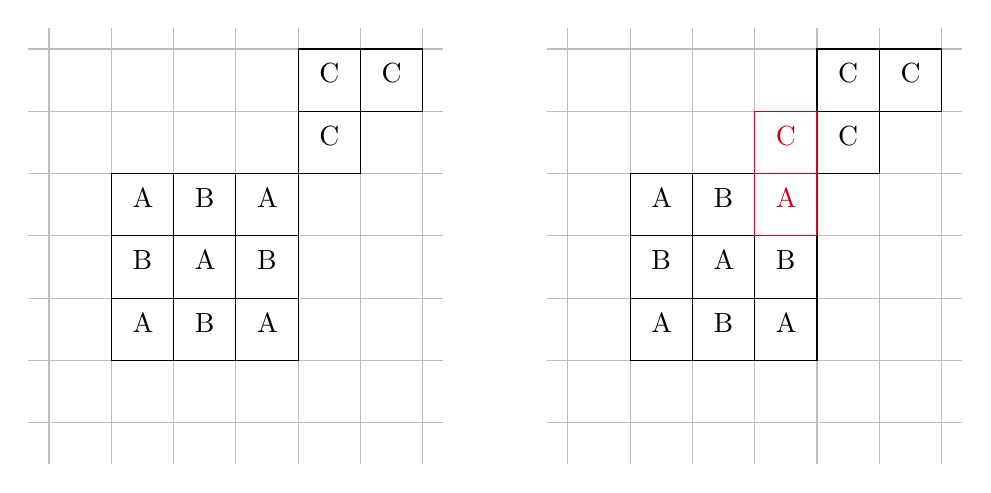
\begin{tikzpicture}[x=0.75pt,y=0.75pt,yscale=-1,xscale=1]
		%uncomment if require: \path (0,300); %set diagram left start at 0, and has height of 300
		
		%Straight Lines [id:da35045523066874695] 
		\draw [color={rgb, 255:red, 190; green, 188; blue, 188 }  ,draw opacity=1 ]   (60,40) -- (60,250) ;
		%Straight Lines [id:da340132848719611] 
		\draw [color={rgb, 255:red, 190; green, 188; blue, 188 }  ,draw opacity=1 ]   (90,40) -- (90,250) ;
		%Straight Lines [id:da9930602253194404] 
		\draw [color={rgb, 255:red, 190; green, 188; blue, 188 }  ,draw opacity=1 ]   (120,40) -- (120,250) ;
		%Straight Lines [id:da673508591738556] 
		\draw [color={rgb, 255:red, 190; green, 188; blue, 188 }  ,draw opacity=1 ]   (150,40) -- (150,250) ;
		%Straight Lines [id:da419114194150617] 
		\draw [color={rgb, 255:red, 190; green, 188; blue, 188 }  ,draw opacity=1 ]   (180,40) -- (180,250) ;
		%Straight Lines [id:da5545224299809445] 
		\draw [color={rgb, 255:red, 190; green, 188; blue, 188 }  ,draw opacity=1 ]   (210,40) -- (210,250) ;
		%Straight Lines [id:da6684800824274905] 
		\draw [color={rgb, 255:red, 190; green, 188; blue, 188 }  ,draw opacity=1 ]   (50,50) -- (250,50) ;
		%Straight Lines [id:da019342059581128557] 
		\draw [color={rgb, 255:red, 190; green, 188; blue, 188 }  ,draw opacity=1 ]   (240,40) -- (240,250) ;
		%Straight Lines [id:da9329975150298714] 
		\draw [color={rgb, 255:red, 190; green, 188; blue, 188 }  ,draw opacity=1 ]   (50,80) -- (250,80) ;
		%Straight Lines [id:da5923754330081309] 
		\draw [color={rgb, 255:red, 190; green, 188; blue, 188 }  ,draw opacity=1 ]   (50,110) -- (250,110) ;
		%Straight Lines [id:da3014815129266917] 
		\draw [color={rgb, 255:red, 190; green, 188; blue, 188 }  ,draw opacity=1 ]   (50,140) -- (250,140) ;
		%Straight Lines [id:da9700279192389916] 
		\draw [color={rgb, 255:red, 190; green, 188; blue, 188 }  ,draw opacity=1 ]   (50,170) -- (250,170) ;
		%Straight Lines [id:da6736918804400827] 
		\draw [color={rgb, 255:red, 190; green, 188; blue, 188 }  ,draw opacity=1 ]   (50,200) -- (250,200) ;
		%Straight Lines [id:da05640786705782641] 
		\draw [color={rgb, 255:red, 190; green, 188; blue, 188 }  ,draw opacity=1 ]   (50,230) -- (250,230) ;
		%Shape: Square [id:dp5803031662244053] 
		\draw   (120,140) -- (150,140) -- (150,170) -- (120,170) -- cycle ;
		
		%Shape: Square [id:dp9196458885257819] 
		\draw   (150,110) -- (180,110) -- (180,140) -- (150,140) -- cycle ;
		
		%Shape: Square [id:dp2648572079254672] 
		\draw   (150,170) -- (180,170) -- (180,200) -- (150,200) -- cycle ;
		
		%Shape: Square [id:dp5425673607779279] 
		\draw   (90,170) -- (120,170) -- (120,200) -- (90,200) -- cycle ;
		
		%Shape: Square [id:dp18348530459906254] 
		\draw   (90,110) -- (120,110) -- (120,140) -- (90,140) -- cycle ;
		
		%Shape: Square [id:dp8856504410510044] 
		\draw   (120,110) -- (150,110) -- (150,140) -- (120,140) -- cycle ;
		
		%Shape: Square [id:dp1873507618967537] 
		\draw   (90,140) -- (120,140) -- (120,170) -- (90,170) -- cycle ;
		
		%Shape: Square [id:dp022117374983126603] 
		\draw   (150,140) -- (180,140) -- (180,170) -- (150,170) -- cycle ;
		
		%Shape: Square [id:dp1634547289103776] 
		\draw   (120,170) -- (150,170) -- (150,200) -- (120,200) -- cycle ;
		
		%Shape: Square [id:dp36442727347773063] 
		\draw   (180,50) -- (210,50) -- (210,80) -- (180,80) -- cycle ;
		%Shape: Square [id:dp5330652912981374] 
		\draw   (210,50) -- (240,50) -- (240,80) -- (210,80) -- cycle ;
		%Shape: Square [id:dp4661865144958631] 
		\draw   (180,80) -- (210,80) -- (210,110) -- (180,110) -- cycle ;
		%Straight Lines [id:da6005649012467171] 
		\draw [color={rgb, 255:red, 190; green, 188; blue, 188 }  ,draw opacity=1 ]   (310,40) -- (310,250) ;
		%Straight Lines [id:da04035283072064799] 
		\draw [color={rgb, 255:red, 190; green, 188; blue, 188 }  ,draw opacity=1 ]   (340,40) -- (340,250) ;
		%Straight Lines [id:da671906501011724] 
		\draw [color={rgb, 255:red, 190; green, 188; blue, 188 }  ,draw opacity=1 ]   (370,40) -- (370,250) ;
		%Straight Lines [id:da49929915066743213] 
		\draw [color={rgb, 255:red, 190; green, 188; blue, 188 }  ,draw opacity=1 ]   (400,40) -- (400,250) ;
		%Straight Lines [id:da6124906908305024] 
		\draw [color={rgb, 255:red, 190; green, 188; blue, 188 }  ,draw opacity=1 ]   (430,40) -- (430,250) ;
		%Straight Lines [id:da17945370773484437] 
		\draw [color={rgb, 255:red, 190; green, 188; blue, 188 }  ,draw opacity=1 ]   (460,40) -- (460,250) ;
		%Straight Lines [id:da6328554243047342] 
		\draw [color={rgb, 255:red, 190; green, 188; blue, 188 }  ,draw opacity=1 ]   (300,50) -- (500,50) ;
		%Straight Lines [id:da6688510350866759] 
		\draw [color={rgb, 255:red, 190; green, 188; blue, 188 }  ,draw opacity=1 ]   (490,40) -- (490,250) ;
		%Straight Lines [id:da612235496519943] 
		\draw [color={rgb, 255:red, 190; green, 188; blue, 188 }  ,draw opacity=1 ]   (300,80) -- (500,80) ;
		%Straight Lines [id:da4514565784776753] 
		\draw [color={rgb, 255:red, 190; green, 188; blue, 188 }  ,draw opacity=1 ]   (300,110) -- (500,110) ;
		%Straight Lines [id:da9360017779771976] 
		\draw [color={rgb, 255:red, 190; green, 188; blue, 188 }  ,draw opacity=1 ]   (300,140) -- (500,140) ;
		%Straight Lines [id:da8873772965675616] 
		\draw [color={rgb, 255:red, 190; green, 188; blue, 188 }  ,draw opacity=1 ]   (300,170) -- (500,170) ;
		%Straight Lines [id:da749590494256885] 
		\draw [color={rgb, 255:red, 190; green, 188; blue, 188 }  ,draw opacity=1 ]   (300,200) -- (500,200) ;
		%Straight Lines [id:da974945622190988] 
		\draw [color={rgb, 255:red, 190; green, 188; blue, 188 }  ,draw opacity=1 ]   (300,230) -- (500,230) ;
		%Shape: Square [id:dp3113813487928936] 
		\draw   (370,140) -- (400,140) -- (400,170) -- (370,170) -- cycle ;
		
		%Shape: Square [id:dp6490479518389014] 
		\draw   (400,170) -- (430,170) -- (430,200) -- (400,200) -- cycle ;
		
		%Shape: Square [id:dp39859172546594845] 
		\draw   (340,170) -- (370,170) -- (370,200) -- (340,200) -- cycle ;
		
		%Shape: Square [id:dp2225864237176991] 
		\draw   (340,110) -- (370,110) -- (370,140) -- (340,140) -- cycle ;
		
		%Shape: Square [id:dp7921412678362084] 
		\draw   (370,110) -- (400,110) -- (400,140) -- (370,140) -- cycle ;
		
		%Shape: Square [id:dp6449792794581529] 
		\draw   (340,140) -- (370,140) -- (370,170) -- (340,170) -- cycle ;
		
		%Shape: Square [id:dp10628620173289283] 
		\draw   (400,140) -- (430,140) -- (430,170) -- (400,170) -- cycle ;
		
		%Shape: Square [id:dp14519260765485775] 
		\draw   (370,170) -- (400,170) -- (400,200) -- (370,200) -- cycle ;
		
		%Shape: Square [id:dp3804583310680284] 
		\draw   (430,50) -- (460,50) -- (460,80) -- (430,80) -- cycle ;
		%Shape: Square [id:dp8462651005127663] 
		\draw   (460,50) -- (490,50) -- (490,80) -- (460,80) -- cycle ;
		%Shape: Square [id:dp23845380767750257] 
		\draw   (430,80) -- (460,80) -- (460,110) -- (430,110) -- cycle ;
		%Shape: Square [id:dp21222113434847067] 
		\draw  [color={rgb, 255:red, 208; green, 2; blue, 27 }  ,draw opacity=1 ] (400,80) -- (430,80) -- (430,110) -- (400,110) -- cycle ;
		%Shape: Square [id:dp188598855194557] 
		\draw  [color={rgb, 255:red, 208; green, 2; blue, 27 }  ,draw opacity=1 ] (400,110) -- (430,110) -- (430,140) -- (400,140) -- cycle ;
		
		
		% Text Node
		\draw (129,146) node [anchor=north west][inner sep=0.75pt]   [align=left] {A};
		% Text Node
		\draw (159,116) node [anchor=north west][inner sep=0.75pt]   [align=left] {A};
		% Text Node
		\draw (159,176) node [anchor=north west][inner sep=0.75pt]   [align=left] {A};
		% Text Node
		\draw (99,176) node [anchor=north west][inner sep=0.75pt]   [align=left] {A};
		% Text Node
		\draw (99,116) node [anchor=north west][inner sep=0.75pt]   [align=left] {A};
		% Text Node
		\draw (129,116) node [anchor=north west][inner sep=0.75pt]   [align=left] {B};
		% Text Node
		\draw (99,146) node [anchor=north west][inner sep=0.75pt]   [align=left] {B};
		% Text Node
		\draw (159,146) node [anchor=north west][inner sep=0.75pt]   [align=left] {B};
		% Text Node
		\draw (129,176) node [anchor=north west][inner sep=0.75pt]   [align=left] {B};
		% Text Node
		\draw (189,56) node [anchor=north west][inner sep=0.75pt]   [align=left] {C};
		% Text Node
		\draw (219,56) node [anchor=north west][inner sep=0.75pt]   [align=left] {C};
		% Text Node
		\draw (189,86) node [anchor=north west][inner sep=0.75pt]   [align=left] {C};
		% Text Node
		\draw (439,56) node [anchor=north west][inner sep=0.75pt]   [align=left] {C};
		% Text Node
		\draw (469,56) node [anchor=north west][inner sep=0.75pt]   [align=left] {C};
		% Text Node
		\draw (439,86) node [anchor=north west][inner sep=0.75pt]   [align=left] {C};
		% Text Node
		\draw (379,176) node [anchor=north west][inner sep=0.75pt]   [align=left] {B};
		% Text Node
		\draw (409,146) node [anchor=north west][inner sep=0.75pt]   [align=left] {B};
		% Text Node
		\draw (349,146) node [anchor=north west][inner sep=0.75pt]   [align=left] {B};
		% Text Node
		\draw (379,116) node [anchor=north west][inner sep=0.75pt]   [align=left] {B};
		% Text Node
		\draw (349,116) node [anchor=north west][inner sep=0.75pt]   [align=left] {A};
		% Text Node
		\draw (349,176) node [anchor=north west][inner sep=0.75pt]   [align=left] {A};
		% Text Node
		\draw (409,176) node [anchor=north west][inner sep=0.75pt]   [align=left] {A};
		% Text Node
		\draw (409,116) node [anchor=north west][inner sep=0.75pt]   [align=left] {\textcolor[rgb]{0.82,0.01,0.11}{A}};
		% Text Node
		\draw (379,146) node [anchor=north west][inner sep=0.75pt]   [align=left] {A};
		% Text Node
		\draw (409,86) node [anchor=north west][inner sep=0.75pt]  [color={rgb, 255:red, 208; green, 2; blue, 27 }  ,opacity=1 ] [align=left] {C};
		
		
	\end{tikzpicture}
\end{figure}
	
	\FloatBarrier
	
	So given the intuition above, one can come up with the following theorem
	
	\begin{theorem}
		In the tiling problem above, a tiling is valid, if and only if its corresponding tiling function is continuous.
	\end{theorem}
	
	
	
	\begin{remark}
		One possible way to formulate this is to assume a discrete topology on $ \Z^2 $, which will force every tiling map to be continuous. However, then, the tiling maps corresponding to valid tiling will precisely be the open maps (the maps that the image of open sets are open sets). 
	\end{remark}
	
	
	\section{Tiles with Glue}
	
	In the example above, we only considered some that some of them want to sit with some other ones and do not sit with certain other ones. However, the way that the tiling problem is formulated in the literature is to assume tiles with different combination of glue values on the sides. I think I can convert this problem to the one similar to above, by considering a sufficiently large product space that captures glue-glue interactions. I know that each glue glue interaction can be captured by a matrix, but I an not certain how to define approporiate topology to convert this formulation to the one similar to above.
	
	
	\subsection{One Possible Formulation}
	Let's assume that the set of all possible glues types is given as alphabet $ G $. For instance, if we have 3 types of glue, then one has $ G = \{g_1,g_2,g_3\} $. Assuming that we work in a 2d grid, consider $ T = G^4 $ or equivalently the set of all strings composed of alphabet in $ G $. For instance, if $ G $ is as given above, then
	\[ \mathcal{T} = \{ g_1g_1g_1g_1,\ g_1g_1g_1g_2,\ g_1g_1g_2g_1,\cdots, g_3g_3g_3g_3. \} \]
	This is the set of all possible tiles. Note that given a combination of glue alphabet, we might not have all of the tiles in $ \mathcal{T} $. For instance, for $ G $ as given above, in one problem we might have only two tiles. For instance:
	\begin{figure}[h!]
	\centering
	
	
	\tikzset{every picture/.style={line width=0.75pt}} %set default line width to 0.75pt        
	
	\begin{tikzpicture}[x=0.75pt,y=0.75pt,yscale=-1,xscale=1]
		%uncomment if require: \path (0,300); %set diagram left start at 0, and has height of 300
		
		%Shape: Square [id:dp14909296198340416] 
		\draw   (170,90) -- (220,90) -- (220,140) -- (170,140) -- cycle ;
		%Shape: Square [id:dp0035098982066744666] 
		\draw   (283,90) -- (333,90) -- (333,140) -- (283,140) -- cycle ;
		
		% Text Node
		\draw (191,76.4) node [anchor=north west][inner sep=0.75pt]  [font=\scriptsize]  {$g_{1}$};
		% Text Node
		\draw (223,106.4) node [anchor=north west][inner sep=0.75pt]  [font=\scriptsize]  {$g_{1}$};
		% Text Node
		\draw (191,138.4) node [anchor=north west][inner sep=0.75pt]  [font=\scriptsize]  {$g_{2}$};
		% Text Node
		\draw (156,106.4) node [anchor=north west][inner sep=0.75pt]  [font=\scriptsize]  {$g_{2}$};
		% Text Node
		\draw (304,76.4) node [anchor=north west][inner sep=0.75pt]  [font=\scriptsize]  {$g_{2}$};
		% Text Node
		\draw (336,106.4) node [anchor=north west][inner sep=0.75pt]  [font=\scriptsize]  {$g_{3}$};
		% Text Node
		\draw (304,138.4) node [anchor=north west][inner sep=0.75pt]  [font=\scriptsize]  {$g_{1}$};
		% Text Node
		\draw (269,106.4) node [anchor=north west][inner sep=0.75pt]  [font=\scriptsize]  {$g_{3}$};
		
		
	\end{tikzpicture}
\end{figure}
	
	Observe that if we assume that these tiles are floating in some kind of solution, thus can rotation, then the tiles corresponding to the codes $ g_1g_2g_2g_1,\ g_2g_2g_1g_1,\ g_2g_1g_1g_2 $ as well as $ g_3g_1g_3g_2,\ g_1g_3g_2g_3,\ g_3g_2g_3g_1  $ will be possible tiles as well. And if tiles can also flip, then all of the permutations in the dihedral group $ D_4 $ will also be possible tiles. In any case, denote the set of all available tiles as $ T \subset\mathcal{T} $. So for the tiles above, that can not rotate nor flip, we have $ T=\{g_1g_1g_2g_2,\ g_2g_3g_1g_3\}. $
		
		
	Given the set of all glue values, then one has a glue strength map $ s: G\times G \to \mathbb{R}_{+} $. It is straight forward to see that this map is symmetric. Given the minimum strength required for two tiles to bind, denoted by $ \tau $, that represents the notion of temperature in aTAM model, we build two directed graphs $ A_h = (T, E_h) $ and $ A_v = (T,E_v) $, where ``h'' and ``v'' stands for horizontal and vertical respectively, and we have used the standard notation for graph $ G=(V,E) $ where $ V $ represents the set of all vertices, and $ E $ represents the set of all edges. 
	
	Now we want to construct the edge sets $ E_h $ and $ E_v $. In words, there is arrow from $ t_1 $ to $ t_2 $ in $ A_v $ if $ t_2 $ can sit on top of $ t_1 $. And similarly, $ t_1 $ is arrowed (?!) to $ t_2 $ if $ t_2 $ can sit on the right side of $ t_1 $. To write this more formally, first observe that when two tiles bind, then the ``North'' part of one touches the ``South'' part of the other one, or, the ``East'' part of one will touch  the ``West'' part of the other tile. Recall that for the tile $ g_1g_1g_2g_2 $, we assume that the glues are represented in the ``North-East-South-West'' order. In the graph $ A_h $, there is an arrow from $ t_1 $ to $ t_2 $ if $ s(t_1(N), t_2(S)) > \tau $. Similarly, there is an arrow from $ t_1 $ to $ t_2 $ in $ A_h $ if $ s(t_1(E),t_2(W)) > \tau $. For instance, for the example above, and assuming $ \tau=1/2 $, assume the following strength matrix for the glue-glue interaction
	\[ s = \begin{pmatrix}
		1 & 0 & 1 \\
		0 & 1 & 0 \\
		1 & 0 & 0
	\end{pmatrix}, \]
	So the directed graph $ A_v $ and $ A_h $ will be
	\begin{figure}[h!]
	\centering
	
	
	
	\tikzset{every picture/.style={line width=0.75pt}} %set default line width to 0.75pt        
	
	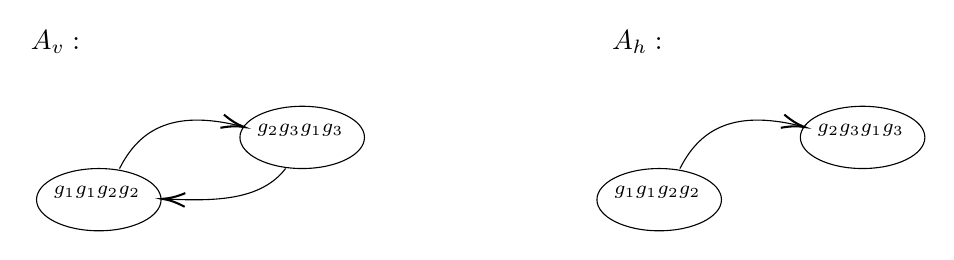
\begin{tikzpicture}[x=0.75pt,y=0.75pt,yscale=-1,xscale=1]
		%uncomment if require: \path (0,300); %set diagram left start at 0, and has height of 300
		
		%Shape: Ellipse [id:dp3480476979550604] 
		\draw   (140,115) .. controls (140,106.72) and (153.43,100) .. (170,100) .. controls (186.57,100) and (200,106.72) .. (200,115) .. controls (200,123.28) and (186.57,130) .. (170,130) .. controls (153.43,130) and (140,123.28) .. (140,115) -- cycle ;
		%Shape: Ellipse [id:dp9456474739758407] 
		\draw   (238,85) .. controls (238,76.72) and (251.43,70) .. (268,70) .. controls (284.57,70) and (298,76.72) .. (298,85) .. controls (298,93.28) and (284.57,100) .. (268,100) .. controls (251.43,100) and (238,93.28) .. (238,85) -- cycle ;
		%Shape: Ellipse [id:dp2502651910875927] 
		\draw   (410,115) .. controls (410,106.72) and (423.43,100) .. (440,100) .. controls (456.57,100) and (470,106.72) .. (470,115) .. controls (470,123.28) and (456.57,130) .. (440,130) .. controls (423.43,130) and (410,123.28) .. (410,115) -- cycle ;
		%Shape: Ellipse [id:dp3792185411216099] 
		\draw   (508,85) .. controls (508,76.72) and (521.43,70) .. (538,70) .. controls (554.57,70) and (568,76.72) .. (568,85) .. controls (568,93.28) and (554.57,100) .. (538,100) .. controls (521.43,100) and (508,93.28) .. (508,85) -- cycle ;
		%Curve Lines [id:da7858938212358939] 
		\draw    (180,100) .. controls (188.87,82.47) and (204.13,70.95) .. (238.42,79.59) ;
		\draw [shift={(240,80)}, rotate = 194.87] [color={rgb, 255:red, 0; green, 0; blue, 0 }  ][line width=0.75]    (10.93,-3.29) .. controls (6.95,-1.4) and (3.31,-0.3) .. (0,0) .. controls (3.31,0.3) and (6.95,1.4) .. (10.93,3.29)   ;
		%Curve Lines [id:da7351349882046846] 
		\draw    (260,100) .. controls (248.11,115.41) and (226.13,115.79) .. (202.43,114.69) ;
		\draw [shift={(200.6,114.6)}, rotate = 2.82] [color={rgb, 255:red, 0; green, 0; blue, 0 }  ][line width=0.75]    (10.93,-3.29) .. controls (6.95,-1.4) and (3.31,-0.3) .. (0,0) .. controls (3.31,0.3) and (6.95,1.4) .. (10.93,3.29)   ;
		%Curve Lines [id:da48287324374825746] 
		\draw    (450,100) .. controls (458.87,82.47) and (474.13,70.95) .. (508.42,79.59) ;
		\draw [shift={(510,80)}, rotate = 194.87] [color={rgb, 255:red, 0; green, 0; blue, 0 }  ][line width=0.75]    (10.93,-3.29) .. controls (6.95,-1.4) and (3.31,-0.3) .. (0,0) .. controls (3.31,0.3) and (6.95,1.4) .. (10.93,3.29)   ;
		
		% Text Node
		\draw (147,107.4) node [anchor=north west][inner sep=0.75pt]  [font=\scriptsize]  {$g_{1} g_{1} g_{2} g_{2}$};
		% Text Node
		\draw (245,77.4) node [anchor=north west][inner sep=0.75pt]  [font=\scriptsize]  {$g_{2} g_{3} g_{1} g_{3}$};
		% Text Node
		\draw (417,107.4) node [anchor=north west][inner sep=0.75pt]  [font=\scriptsize]  {$g_{1} g_{1} g_{2} g_{2}$};
		% Text Node
		\draw (515,77.4) node [anchor=north west][inner sep=0.75pt]  [font=\scriptsize]  {$g_{2} g_{3} g_{1} g_{3}$};
		% Text Node
		\draw (136,32.4) node [anchor=north west][inner sep=0.75pt]    {$A_{v} :$};
		% Text Node
		\draw (416,32.4) node [anchor=north west][inner sep=0.75pt]    {$A_{h} :$};
		
		
	\end{tikzpicture}
\end{figure}
	
	For the sake of completeness, assuming the possibility of rotation, then the set of possible tiles will be
	\begin{figure}[h!]
	\centering
	
	\tikzset{every picture/.style={line width=0.75pt}} %set default line width to 0.75pt        
	
	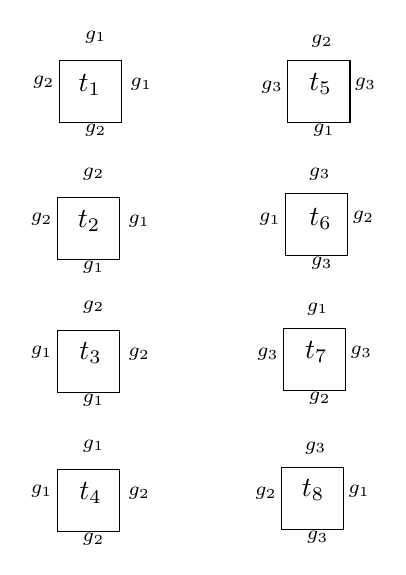
\begin{tikzpicture}[x=0.75pt,y=0.75pt,yscale=-1,xscale=1]
		%uncomment if require: \path (0,300); %set diagram left start at 0, and has height of 300
		
		%Shape: Square [id:dp22532401478603215] 
		\draw   (143,40) -- (173,40) -- (173,70) -- (143,70) -- cycle ;
		%Shape: Square [id:dp09979375032138338] 
		\draw   (253,40) -- (283,40) -- (283,70) -- (253,70) -- cycle ;
		%Shape: Square [id:dp3168351739514086] 
		\draw   (142,106) -- (172,106) -- (172,136) -- (142,136) -- cycle ;
		%Shape: Square [id:dp8233768301251638] 
		\draw   (142,170) -- (172,170) -- (172,200) -- (142,200) -- cycle ;
		%Shape: Square [id:dp752708971833606] 
		\draw   (142,237) -- (172,237) -- (172,267) -- (142,267) -- cycle ;
		%Shape: Square [id:dp5808750315542068] 
		\draw   (252,104) -- (282,104) -- (282,134) -- (252,134) -- cycle ;
		%Shape: Square [id:dp3802022570055066] 
		\draw   (251,169) -- (281,169) -- (281,199) -- (251,199) -- cycle ;
		%Shape: Square [id:dp6621336678331176] 
		\draw   (250,236) -- (280,236) -- (280,266) -- (250,266) -- cycle ;
		
		% Text Node
		\draw (154,24.4) node [anchor=north west][inner sep=0.75pt]  [font=\scriptsize]  {$g_{1}$};
		% Text Node
		\draw (176,47.4) node [anchor=north west][inner sep=0.75pt]  [font=\scriptsize]  {$g_{1}$};
		% Text Node
		\draw (154,69.4) node [anchor=north west][inner sep=0.75pt]  [font=\scriptsize]  {$g_{2}$};
		% Text Node
		\draw (129,46.4) node [anchor=north west][inner sep=0.75pt]  [font=\scriptsize]  {$g_{2}$};
		% Text Node
		\draw (263,26.4) node [anchor=north west][inner sep=0.75pt]  [font=\scriptsize]  {$g_{2}$};
		% Text Node
		\draw (284,47.4) node [anchor=north west][inner sep=0.75pt]  [font=\scriptsize]  {$g_{3}$};
		% Text Node
		\draw (264,69.4) node [anchor=north west][inner sep=0.75pt]  [font=\scriptsize]  {$g_{1}$};
		% Text Node
		\draw (239,48.4) node [anchor=north west][inner sep=0.75pt]  [font=\scriptsize]  {$g_{3}$};
		% Text Node
		\draw (153,90.4) node [anchor=north west][inner sep=0.75pt]  [font=\scriptsize]  {$g_{2}$};
		% Text Node
		\draw (175,113.4) node [anchor=north west][inner sep=0.75pt]  [font=\scriptsize]  {$g_{1}$};
		% Text Node
		\draw (153,135.4) node [anchor=north west][inner sep=0.75pt]  [font=\scriptsize]  {$g_{1}$};
		% Text Node
		\draw (128,112.4) node [anchor=north west][inner sep=0.75pt]  [font=\scriptsize]  {$g_{2}$};
		% Text Node
		\draw (153,154.4) node [anchor=north west][inner sep=0.75pt]  [font=\scriptsize]  {$g_{2}$};
		% Text Node
		\draw (175,177.4) node [anchor=north west][inner sep=0.75pt]  [font=\scriptsize]  {$g_{2}$};
		% Text Node
		\draw (153,199.4) node [anchor=north west][inner sep=0.75pt]  [font=\scriptsize]  {$g_{1}$};
		% Text Node
		\draw (128,176.4) node [anchor=north west][inner sep=0.75pt]  [font=\scriptsize]  {$g_{1}$};
		% Text Node
		\draw (153,221.4) node [anchor=north west][inner sep=0.75pt]  [font=\scriptsize]  {$g_{1}$};
		% Text Node
		\draw (175,244.4) node [anchor=north west][inner sep=0.75pt]  [font=\scriptsize]  {$g_{2}$};
		% Text Node
		\draw (153,266.4) node [anchor=north west][inner sep=0.75pt]  [font=\scriptsize]  {$g_{2}$};
		% Text Node
		\draw (128,243.4) node [anchor=north west][inner sep=0.75pt]  [font=\scriptsize]  {$g_{1}$};
		% Text Node
		\draw (262,90.4) node [anchor=north west][inner sep=0.75pt]  [font=\scriptsize]  {$g_{3}$};
		% Text Node
		\draw (283,111.4) node [anchor=north west][inner sep=0.75pt]  [font=\scriptsize]  {$g_{2}$};
		% Text Node
		\draw (263,133.4) node [anchor=north west][inner sep=0.75pt]  [font=\scriptsize]  {$g_{3}$};
		% Text Node
		\draw (238,112.4) node [anchor=north west][inner sep=0.75pt]  [font=\scriptsize]  {$g_{1}$};
		% Text Node
		\draw (261,155.4) node [anchor=north west][inner sep=0.75pt]  [font=\scriptsize]  {$g_{1}$};
		% Text Node
		\draw (282,176.4) node [anchor=north west][inner sep=0.75pt]  [font=\scriptsize]  {$g_{3}$};
		% Text Node
		\draw (262,198.4) node [anchor=north west][inner sep=0.75pt]  [font=\scriptsize]  {$g_{2}$};
		% Text Node
		\draw (237,177.4) node [anchor=north west][inner sep=0.75pt]  [font=\scriptsize]  {$g_{3}$};
		% Text Node
		\draw (260,222.4) node [anchor=north west][inner sep=0.75pt]  [font=\scriptsize]  {$g_{3}$};
		% Text Node
		\draw (281,243.4) node [anchor=north west][inner sep=0.75pt]  [font=\scriptsize]  {$g_{1}$};
		% Text Node
		\draw (261,265.4) node [anchor=north west][inner sep=0.75pt]  [font=\scriptsize]  {$g_{3}$};
		% Text Node
		\draw (236,244.4) node [anchor=north west][inner sep=0.75pt]  [font=\scriptsize]  {$g_{2}$};
		% Text Node
		\draw (151,45.4) node [anchor=north west][inner sep=0.75pt]    {$t_{1}$};
		% Text Node
		\draw (150.6,111) node [anchor=north west][inner sep=0.75pt]    {$t_{2}$};
		% Text Node
		\draw (151.4,174.6) node [anchor=north west][inner sep=0.75pt]    {$t_{3}$};
		% Text Node
		\draw (151.4,241.8) node [anchor=north west][inner sep=0.75pt]    {$t_{4}$};
		% Text Node
		\draw (262.2,45) node [anchor=north west][inner sep=0.75pt]    {$t_{5}$};
		% Text Node
		\draw (262.2,109.8) node [anchor=north west][inner sep=0.75pt]    {$t_{6}$};
		% Text Node
		\draw (260.2,174.2) node [anchor=north west][inner sep=0.75pt]    {$t_{7}$};
		% Text Node
		\draw (258.6,240.6) node [anchor=north west][inner sep=0.75pt]    {$t_{8}$};
		
		
	\end{tikzpicture}
\end{figure}
	
	where for the convenience we have assigned labels for each tile. The $ A_v $ graph for this set of tiles will be as the following graph, where the one on the left is $ A_v $ and the one on the right is $ A_h $.
	
	\begin{figure}[h!]
		\centering
		\includegraphics[width=0.5\linewidth]{images/A_vA_hwithRotation.png}
		\label{fig:graph}
	\end{figure}
	\FloatBarrier
	The computation of these graphs might seem tedious at first glance, however, it is easy to calculate them even by hand. I am yet to think on how to do this algorithmic, but for now I am doing the computations by hand. Here I will explain the simple ``manual'' way to do this, and in the next subsection I will highlight how to use some group theory to make the calculation simpler.
	
	First, we start by constructing $ A_v $. To do this, observe that those tiles that their top edge is $ g_1 $, the tiles that their bottom glue is $ g_1 $ or $ g_3 $ can attach to them (i.e. there will be an arrow from the tile with top glue $ g_1 $ to the tiles that their bottom glue is $ g_1 $ or $ g_3 $). Observe that the tiles $ t_1,t_4 $, and $ t_7 $ all have similar top glue, $ g_1 $. So 
	\[ \tile{t_1},\tile{t_4}, \tile{t_7} \quad\longrightarrow\quad \tile{t_2},\tile{t_3},\tile{t_5},\tile{t_6},\tile{t_8}, \]
	where the diagram above should be interpreted as ``there is an arrow from each of tile on the LHS to all of the tiles in the RHS''. Furthermore, for those with $ g_2 $ sitting on top, since $ g_2 $ only sits with $ g_2 $, there is an arrow from these tiles to only those tiles that have $ g_2 $ at the bottom. So
	\[ \tile{t_2},\tile{t_3},\tile{t_5} \quad\longrightarrow\quad \tile{t_1},\tile{t_4},\tile{t_7}. \]
	And finally, for those tiles with $ g_3 $ on their top, since $ g_3 $ only sits with $ g_1 $, there is an arrow from these tiles to the tiles that have $ g_1 $ at the bottom. So
	\[ \tile{t_6},\tile{t_8} \quad\longrightarrow\quad \tile{t_2},\tile{t_3},\tile{t_5} \]
	Now one can easily draw the corresponding graph.
	
	We can follow a similar procedure for $ A_h $. Using similar arguments as above (but this time using the fact that there is an arrow from tile $ A $ to tile $ B $ if $ B $ can sit on the right hand side of $ A $). So we will have
%	\begin{align*}
%		\tile{t_1},\tile{t_2},\tile{t_8} &\quad\longrightarrow\quad& \tile{t_3},\tile{t_4},\tile{t_6},\tile{t_7}, \\
%		\tile{t_3},\tile{t_4},\tile{t_6} &\quad\longrightarrow\quad& \tile{t_1},\tile{t_2},\tile{t_8}, \\
%		\tile{t_5},\tile{t_7}             &\quad\longrightarrow\quad& \tile{t_3},\tile{t_4},\tile{t_6}
%	\end{align*}
	\[ \tile{t_1},\tile{t_2},\tile{t_8} \quad\longrightarrow\quad \tile{t_3},\tile{t_4},\tile{t_6},\tile{t_7},\tile{t_5}, \]
	\[ \tile{t_3},\tile{t_4},\tile{t_6} \quad\longrightarrow\quad \tile{t_1},\tile{t_2},\tile{t_8}, \]
	\[ \tile{t_5},\tile{t_7} \quad\longrightarrow\quad \tile{t_3},\tile{t_4},\tile{t_6}. \]
	
	There is also another way to compute the $ A_v $ and $ A_h $ graphs, which reveals its connection to the glue strength matrix.  Let $ E $ and $ W $ (stands for ``East'' and ``West'') denote two equivalence relation on the tile set $ T $, where two tiles are related in the sense of $ E $ (i.e. $ t_1\ E\ t_2 $) iff both of them have same glue type on their right hand side. Similarly, two tiles are related in the sense of $ W $ if and only they have a similar glue on their left hand side. Similarly, let $ N $ and $ S $ be the equivalence relations capturing the similarity of glue types on ``North'' and ``South''. To construct the $ A_v $ graph we need the partitions generated by $ N $ and $ S $, however, for $ A_h $ we need the partitions generated by $ W $ and $ E $. Starting with $ A_v $, first, observe that the relation $ N $ induces the following equivalence classes
	\[ [g_1]_N = \{t_1,t_4,t_7\}, \quad [g_2]_N = \{t_2,t_3,t_5\}, \quad [g_3]_N = \{t_6, t_8\}, \] 
	and for $ B $ we have
	\[ [g_1]_S = \{t_2,t_3,t_5\}, \quad [g_2]_S = \{t_1,t_4,t_7\}, \quad [g_3]_S = \{t_6,t_8\}. \]
	And now construct a graph where the edges are these equivalence relations, and we connect $ [g_i]_N $ with an arrow to $ [g_j]_S $ if $ s(g_i,g_j) > \tau $. In other words, the glue matrix will lead to the following connections between these equivalence relations
	\begin{figure}[h!]
	\centering
	
	
	
	\tikzset{every picture/.style={line width=0.75pt}} %set default line width to 0.75pt        
	
	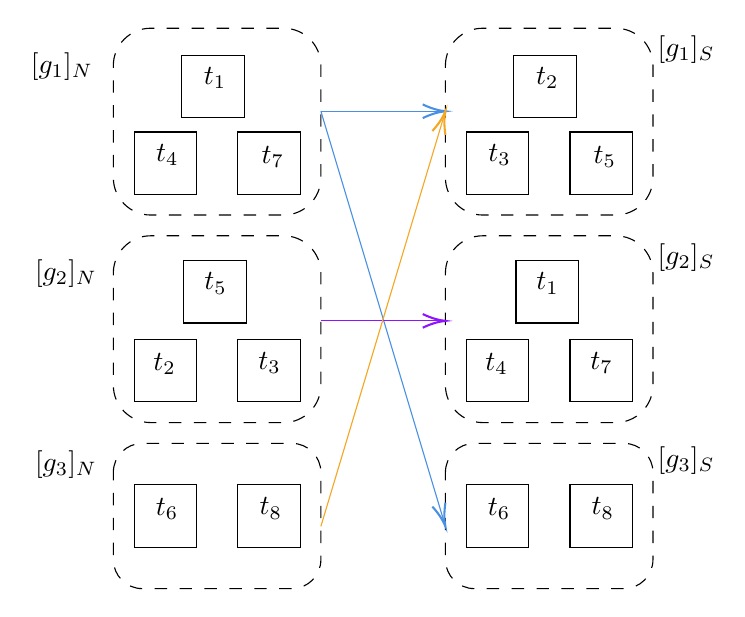
\begin{tikzpicture}[x=0.75pt,y=0.75pt,yscale=-1,xscale=1]
		%uncomment if require: \path (0,300); %set diagram left start at 0, and has height of 300
		
		%Shape: Square [id:dp3671408847760568] 
		\draw   (320,160) -- (350,160) -- (350,190) -- (320,190) -- cycle ;
		%Shape: Square [id:dp3324862746099033] 
		\draw   (370,230) -- (400,230) -- (400,260) -- (370,260) -- cycle ;
		%Shape: Square [id:dp12220174197379818] 
		\draw   (370,160) -- (400,160) -- (400,190) -- (370,190) -- cycle ;
		%Shape: Square [id:dp1297610179609353] 
		\draw   (320,60) -- (350,60) -- (350,90) -- (320,90) -- cycle ;
		
		%Shape: Square [id:dp7523548467624515] 
		\draw   (343,23) -- (373,23) -- (373,53) -- (343,53) -- cycle ;
		%Shape: Square [id:dp5130314226054026] 
		\draw   (370,60) -- (400,60) -- (400,90) -- (370,90) -- cycle ;
		%Shape: Square [id:dp618972762357851] 
		\draw   (320,230) -- (350,230) -- (350,260) -- (320,260) -- cycle ;
		%Shape: Square [id:dp15772738552577148] 
		\draw   (344,122) -- (374,122) -- (374,152) -- (344,152) -- cycle ;
		%Shape: Square [id:dp5693511293927607] 
		\draw   (160,160) -- (190,160) -- (190,190) -- (160,190) -- cycle ;
		%Shape: Square [id:dp3278599549672909] 
		\draw   (210,230) -- (240,230) -- (240,260) -- (210,260) -- cycle ;
		%Shape: Square [id:dp1201027466762743] 
		\draw   (210,160) -- (240,160) -- (240,190) -- (210,190) -- cycle ;
		%Shape: Square [id:dp08271852466340757] 
		\draw   (160,60) -- (190,60) -- (190,90) -- (160,90) -- cycle ;
		
		%Shape: Square [id:dp21363052401120453] 
		\draw   (183,23) -- (213,23) -- (213,53) -- (183,53) -- cycle ;
		%Shape: Square [id:dp732242356691577] 
		\draw   (210,60) -- (240,60) -- (240,90) -- (210,90) -- cycle ;
		%Shape: Square [id:dp15654774282214734] 
		\draw   (160,230) -- (190,230) -- (190,260) -- (160,260) -- cycle ;
		%Shape: Square [id:dp34726784169013514] 
		\draw   (184,122) -- (214,122) -- (214,152) -- (184,152) -- cycle ;
		%Rounded Rect [id:dp01423768550096527] 
		\draw  [dash pattern={on 4.5pt off 4.5pt}] (150,28) .. controls (150,18.06) and (158.06,10) .. (168,10) -- (232,10) .. controls (241.94,10) and (250,18.06) .. (250,28) -- (250,82) .. controls (250,91.94) and (241.94,100) .. (232,100) -- (168,100) .. controls (158.06,100) and (150,91.94) .. (150,82) -- cycle ;
		%Rounded Rect [id:dp023359630662205477] 
		\draw  [dash pattern={on 4.5pt off 4.5pt}] (150,128) .. controls (150,118.06) and (158.06,110) .. (168,110) -- (232,110) .. controls (241.94,110) and (250,118.06) .. (250,128) -- (250,182) .. controls (250,191.94) and (241.94,200) .. (232,200) -- (168,200) .. controls (158.06,200) and (150,191.94) .. (150,182) -- cycle ;
		%Rounded Rect [id:dp5880539252179204] 
		\draw  [dash pattern={on 4.5pt off 4.5pt}] (150,224) .. controls (150,216.27) and (156.27,210) .. (164,210) -- (236,210) .. controls (243.73,210) and (250,216.27) .. (250,224) -- (250,266) .. controls (250,273.73) and (243.73,280) .. (236,280) -- (164,280) .. controls (156.27,280) and (150,273.73) .. (150,266) -- cycle ;
		%Rounded Rect [id:dp37862908048708466] 
		\draw  [dash pattern={on 4.5pt off 4.5pt}] (310,28) .. controls (310,18.06) and (318.06,10) .. (328,10) -- (392,10) .. controls (401.94,10) and (410,18.06) .. (410,28) -- (410,82) .. controls (410,91.94) and (401.94,100) .. (392,100) -- (328,100) .. controls (318.06,100) and (310,91.94) .. (310,82) -- cycle ;
		%Rounded Rect [id:dp2457398001361082] 
		\draw  [dash pattern={on 4.5pt off 4.5pt}] (310,128) .. controls (310,118.06) and (318.06,110) .. (328,110) -- (392,110) .. controls (401.94,110) and (410,118.06) .. (410,128) -- (410,182) .. controls (410,191.94) and (401.94,200) .. (392,200) -- (328,200) .. controls (318.06,200) and (310,191.94) .. (310,182) -- cycle ;
		%Rounded Rect [id:dp03170031338580892] 
		\draw  [dash pattern={on 4.5pt off 4.5pt}] (310,224) .. controls (310,216.27) and (316.27,210) .. (324,210) -- (396,210) .. controls (403.73,210) and (410,216.27) .. (410,224) -- (410,266) .. controls (410,273.73) and (403.73,280) .. (396,280) -- (324,280) .. controls (316.27,280) and (310,273.73) .. (310,266) -- cycle ;
		%Straight Lines [id:da3139663249685024] 
		\draw [color={rgb, 255:red, 74; green, 144; blue, 226 }  ,draw opacity=1 ]   (250,50) -- (308,50) ;
		\draw [shift={(310,50)}, rotate = 180] [color={rgb, 255:red, 74; green, 144; blue, 226 }  ,draw opacity=1 ][line width=0.75]    (10.93,-3.29) .. controls (6.95,-1.4) and (3.31,-0.3) .. (0,0) .. controls (3.31,0.3) and (6.95,1.4) .. (10.93,3.29)   ;
		%Straight Lines [id:da23012772702959772] 
		\draw [color={rgb, 255:red, 74; green, 144; blue, 226 }  ,draw opacity=1 ]   (250,50) -- (309.43,248.08) ;
		\draw [shift={(310,250)}, rotate = 253.3] [color={rgb, 255:red, 74; green, 144; blue, 226 }  ,draw opacity=1 ][line width=0.75]    (10.93,-3.29) .. controls (6.95,-1.4) and (3.31,-0.3) .. (0,0) .. controls (3.31,0.3) and (6.95,1.4) .. (10.93,3.29)   ;
		%Straight Lines [id:da7143198589423927] 
		\draw [color={rgb, 255:red, 144; green, 19; blue, 254 }  ,draw opacity=1 ]   (250,151) -- (308,151) ;
		\draw [shift={(310,151)}, rotate = 180] [color={rgb, 255:red, 144; green, 19; blue, 254 }  ,draw opacity=1 ][line width=0.75]    (10.93,-3.29) .. controls (6.95,-1.4) and (3.31,-0.3) .. (0,0) .. controls (3.31,0.3) and (6.95,1.4) .. (10.93,3.29)   ;
		%Straight Lines [id:da7580479453586497] 
		\draw [color={rgb, 255:red, 245; green, 166; blue, 35 }  ,draw opacity=1 ]   (250,250) -- (309.43,51.92) ;
		\draw [shift={(310,50)}, rotate = 106.7] [color={rgb, 255:red, 245; green, 166; blue, 35 }  ,draw opacity=1 ][line width=0.75]    (10.93,-3.29) .. controls (6.95,-1.4) and (3.31,-0.3) .. (0,0) .. controls (3.31,0.3) and (6.95,1.4) .. (10.93,3.29)   ;
		
		% Text Node
		\draw (328,165.4) node [anchor=north west][inner sep=0.75pt]    {$t_{4}$};
		% Text Node
		\draw (378.6,165) node [anchor=north west][inner sep=0.75pt]    {$t_{7}$};
		% Text Node
		\draw (352.4,27.8) node [anchor=north west][inner sep=0.75pt]    {$t_{2}$};
		% Text Node
		\draw (379.2,235) node [anchor=north west][inner sep=0.75pt]    {$t_{8}$};
		% Text Node
		\draw (380.2,65.8) node [anchor=north west][inner sep=0.75pt]    {$t_{5}$};
		% Text Node
		\draw (329.2,235.2) node [anchor=north west][inner sep=0.75pt]    {$t_{6}$};
		% Text Node
		\draw (352.6,126.6) node [anchor=north west][inner sep=0.75pt]    {$t_{1}$};
		% Text Node
		\draw (329.4,64.6) node [anchor=north west][inner sep=0.75pt]    {$t_{3}$};
		% Text Node
		\draw (168,165.4) node [anchor=north west][inner sep=0.75pt]    {$t_{2}$};
		% Text Node
		\draw (218.6,165) node [anchor=north west][inner sep=0.75pt]    {$t_{3}$};
		% Text Node
		\draw (192.4,27.8) node [anchor=north west][inner sep=0.75pt]    {$t_{1}$};
		% Text Node
		\draw (219.2,235) node [anchor=north west][inner sep=0.75pt]    {$t_{8}$};
		% Text Node
		\draw (220.2,65.8) node [anchor=north west][inner sep=0.75pt]    {$t_{7}$};
		% Text Node
		\draw (169.2,235.2) node [anchor=north west][inner sep=0.75pt]    {$t_{6}$};
		% Text Node
		\draw (192.6,126.6) node [anchor=north west][inner sep=0.75pt]    {$t_{5}$};
		% Text Node
		\draw (169.4,64.6) node [anchor=north west][inner sep=0.75pt]    {$t_{4}$};
		% Text Node
		\draw (109,20.4) node [anchor=north west][inner sep=0.75pt]    {$[ g_{1}]_{N}$};
		% Text Node
		\draw (111,120.4) node [anchor=north west][inner sep=0.75pt]    {$[ g_{2}]_{N}$};
		% Text Node
		\draw (111,212.4) node [anchor=north west][inner sep=0.75pt]    {$[ g_{3}]_{N}$};
		% Text Node
		\draw (411,12.4) node [anchor=north west][inner sep=0.75pt]    {$[ g_{1}]_{S}$};
		% Text Node
		\draw (411,112.4) node [anchor=north west][inner sep=0.75pt]    {$[ g_{2}]_{S}$};
		% Text Node
		\draw (411,210.4) node [anchor=north west][inner sep=0.75pt]    {$[ g_{3}]_{S}$};
		
		
	\end{tikzpicture}
\end{figure}
	\FloatBarrier
	Similarly, the $ E $ and $ W $ relations will lead to the following partitions:
	\[ [g_1]_E = \{t_1,t_2,t_8\}, \quad [g_2]_E = \{t_3,t_4,t_6\}, \quad [g_3]_E = \{t_5,t_7\}, \]
	and
	\[ [g_1]_W = \{t_3,t_4,t_6\}, \quad [g_2]_W = \{t_1,t_2,t_8\}, \quad [g_3]_W = \{t_7, t_5\} \]
	where the corresponding diagram including the connections will be
	\begin{figure}[h!]
	\centering
	
	
	\tikzset{every picture/.style={line width=0.75pt}} %set default line width to 0.75pt        
	
	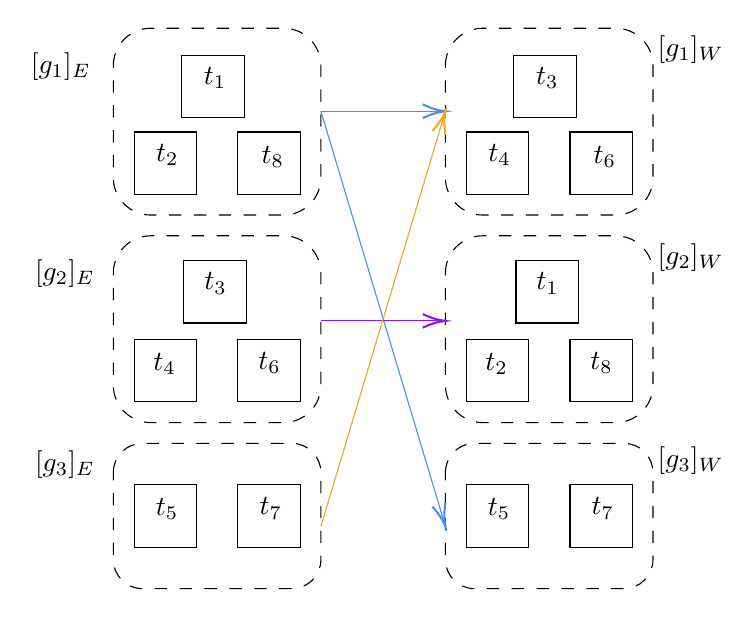
\begin{tikzpicture}[x=0.75pt,y=0.75pt,yscale=-1,xscale=1]
		%uncomment if require: \path (0,300); %set diagram left start at 0, and has height of 300
		
		%Shape: Square [id:dp9827031405699634] 
		\draw   (320,160) -- (350,160) -- (350,190) -- (320,190) -- cycle ;
		%Shape: Square [id:dp8023961227081475] 
		\draw   (370,230) -- (400,230) -- (400,260) -- (370,260) -- cycle ;
		%Shape: Square [id:dp03712561702321415] 
		\draw   (370,160) -- (400,160) -- (400,190) -- (370,190) -- cycle ;
		%Shape: Square [id:dp665252748842778] 
		\draw   (320,60) -- (350,60) -- (350,90) -- (320,90) -- cycle ;
		
		%Shape: Square [id:dp8558270957306437] 
		\draw   (343,23) -- (373,23) -- (373,53) -- (343,53) -- cycle ;
		%Shape: Square [id:dp7592436585314244] 
		\draw   (370,60) -- (400,60) -- (400,90) -- (370,90) -- cycle ;
		%Shape: Square [id:dp5096150167457512] 
		\draw   (320,230) -- (350,230) -- (350,260) -- (320,260) -- cycle ;
		%Shape: Square [id:dp468896653565648] 
		\draw   (344,122) -- (374,122) -- (374,152) -- (344,152) -- cycle ;
		%Shape: Square [id:dp5959228737950086] 
		\draw   (160,160) -- (190,160) -- (190,190) -- (160,190) -- cycle ;
		%Shape: Square [id:dp4137689515105887] 
		\draw   (210,230) -- (240,230) -- (240,260) -- (210,260) -- cycle ;
		%Shape: Square [id:dp2890656867000987] 
		\draw   (210,160) -- (240,160) -- (240,190) -- (210,190) -- cycle ;
		%Shape: Square [id:dp2222867301895708] 
		\draw   (160,60) -- (190,60) -- (190,90) -- (160,90) -- cycle ;
		
		%Shape: Square [id:dp9529971943334293] 
		\draw   (183,23) -- (213,23) -- (213,53) -- (183,53) -- cycle ;
		%Shape: Square [id:dp3186523365427516] 
		\draw   (210,60) -- (240,60) -- (240,90) -- (210,90) -- cycle ;
		%Shape: Square [id:dp6108775427683606] 
		\draw   (160,230) -- (190,230) -- (190,260) -- (160,260) -- cycle ;
		%Shape: Square [id:dp4159406011644433] 
		\draw   (184,122) -- (214,122) -- (214,152) -- (184,152) -- cycle ;
		%Rounded Rect [id:dp6633339374263201] 
		\draw  [dash pattern={on 4.5pt off 4.5pt}] (150,28) .. controls (150,18.06) and (158.06,10) .. (168,10) -- (232,10) .. controls (241.94,10) and (250,18.06) .. (250,28) -- (250,82) .. controls (250,91.94) and (241.94,100) .. (232,100) -- (168,100) .. controls (158.06,100) and (150,91.94) .. (150,82) -- cycle ;
		%Rounded Rect [id:dp07771024867524312] 
		\draw  [dash pattern={on 4.5pt off 4.5pt}] (150,128) .. controls (150,118.06) and (158.06,110) .. (168,110) -- (232,110) .. controls (241.94,110) and (250,118.06) .. (250,128) -- (250,182) .. controls (250,191.94) and (241.94,200) .. (232,200) -- (168,200) .. controls (158.06,200) and (150,191.94) .. (150,182) -- cycle ;
		%Rounded Rect [id:dp03141626075041437] 
		\draw  [dash pattern={on 4.5pt off 4.5pt}] (150,224) .. controls (150,216.27) and (156.27,210) .. (164,210) -- (236,210) .. controls (243.73,210) and (250,216.27) .. (250,224) -- (250,266) .. controls (250,273.73) and (243.73,280) .. (236,280) -- (164,280) .. controls (156.27,280) and (150,273.73) .. (150,266) -- cycle ;
		%Rounded Rect [id:dp5622046683031108] 
		\draw  [dash pattern={on 4.5pt off 4.5pt}] (310,28) .. controls (310,18.06) and (318.06,10) .. (328,10) -- (392,10) .. controls (401.94,10) and (410,18.06) .. (410,28) -- (410,82) .. controls (410,91.94) and (401.94,100) .. (392,100) -- (328,100) .. controls (318.06,100) and (310,91.94) .. (310,82) -- cycle ;
		%Rounded Rect [id:dp20845445372702165] 
		\draw  [dash pattern={on 4.5pt off 4.5pt}] (310,128) .. controls (310,118.06) and (318.06,110) .. (328,110) -- (392,110) .. controls (401.94,110) and (410,118.06) .. (410,128) -- (410,182) .. controls (410,191.94) and (401.94,200) .. (392,200) -- (328,200) .. controls (318.06,200) and (310,191.94) .. (310,182) -- cycle ;
		%Rounded Rect [id:dp061768139424575264] 
		\draw  [dash pattern={on 4.5pt off 4.5pt}] (310,224) .. controls (310,216.27) and (316.27,210) .. (324,210) -- (396,210) .. controls (403.73,210) and (410,216.27) .. (410,224) -- (410,266) .. controls (410,273.73) and (403.73,280) .. (396,280) -- (324,280) .. controls (316.27,280) and (310,273.73) .. (310,266) -- cycle ;
		%Straight Lines [id:da06878187278722059] 
		\draw [color={rgb, 255:red, 74; green, 144; blue, 226 }  ,draw opacity=1 ]   (250,50) -- (308,50) ;
		\draw [shift={(310,50)}, rotate = 180] [color={rgb, 255:red, 74; green, 144; blue, 226 }  ,draw opacity=1 ][line width=0.75]    (10.93,-3.29) .. controls (6.95,-1.4) and (3.31,-0.3) .. (0,0) .. controls (3.31,0.3) and (6.95,1.4) .. (10.93,3.29)   ;
		%Straight Lines [id:da03355516067793607] 
		\draw [color={rgb, 255:red, 74; green, 144; blue, 226 }  ,draw opacity=1 ]   (250,50) -- (309.43,248.08) ;
		\draw [shift={(310,250)}, rotate = 253.3] [color={rgb, 255:red, 74; green, 144; blue, 226 }  ,draw opacity=1 ][line width=0.75]    (10.93,-3.29) .. controls (6.95,-1.4) and (3.31,-0.3) .. (0,0) .. controls (3.31,0.3) and (6.95,1.4) .. (10.93,3.29)   ;
		%Straight Lines [id:da18343296273423393] 
		\draw [color={rgb, 255:red, 144; green, 19; blue, 254 }  ,draw opacity=1 ]   (250,151) -- (308,151) ;
		\draw [shift={(310,151)}, rotate = 180] [color={rgb, 255:red, 144; green, 19; blue, 254 }  ,draw opacity=1 ][line width=0.75]    (10.93,-3.29) .. controls (6.95,-1.4) and (3.31,-0.3) .. (0,0) .. controls (3.31,0.3) and (6.95,1.4) .. (10.93,3.29)   ;
		%Straight Lines [id:da707149216624745] 
		\draw [color={rgb, 255:red, 245; green, 166; blue, 35 }  ,draw opacity=1 ]   (250,250) -- (309.43,51.92) ;
		\draw [shift={(310,50)}, rotate = 106.7] [color={rgb, 255:red, 245; green, 166; blue, 35 }  ,draw opacity=1 ][line width=0.75]    (10.93,-3.29) .. controls (6.95,-1.4) and (3.31,-0.3) .. (0,0) .. controls (3.31,0.3) and (6.95,1.4) .. (10.93,3.29)   ;
		
		% Text Node
		\draw (328,165.4) node [anchor=north west][inner sep=0.75pt]    {$t_{2}$};
		% Text Node
		\draw (378.6,165) node [anchor=north west][inner sep=0.75pt]    {$t_{8}$};
		% Text Node
		\draw (352.4,27.8) node [anchor=north west][inner sep=0.75pt]    {$t_{3}$};
		% Text Node
		\draw (379.2,235) node [anchor=north west][inner sep=0.75pt]    {$t_{7}$};
		% Text Node
		\draw (380.2,65.8) node [anchor=north west][inner sep=0.75pt]    {$t_{6}$};
		% Text Node
		\draw (329.2,235.2) node [anchor=north west][inner sep=0.75pt]    {$t_{5}$};
		% Text Node
		\draw (352.6,126.6) node [anchor=north west][inner sep=0.75pt]    {$t_{1}$};
		% Text Node
		\draw (329.4,64.6) node [anchor=north west][inner sep=0.75pt]    {$t_{4}$};
		% Text Node
		\draw (168,165.4) node [anchor=north west][inner sep=0.75pt]    {$t_{4}$};
		% Text Node
		\draw (218.6,165) node [anchor=north west][inner sep=0.75pt]    {$t_{6}$};
		% Text Node
		\draw (192.4,27.8) node [anchor=north west][inner sep=0.75pt]    {$t_{1}$};
		% Text Node
		\draw (219.2,235) node [anchor=north west][inner sep=0.75pt]    {$t_{7}$};
		% Text Node
		\draw (220.2,65.8) node [anchor=north west][inner sep=0.75pt]    {$t_{8}$};
		% Text Node
		\draw (169.2,235.2) node [anchor=north west][inner sep=0.75pt]    {$t_{5}$};
		% Text Node
		\draw (192.6,126.6) node [anchor=north west][inner sep=0.75pt]    {$t_{3}$};
		% Text Node
		\draw (169.4,64.6) node [anchor=north west][inner sep=0.75pt]    {$t_{2}$};
		% Text Node
		\draw (109,20.4) node [anchor=north west][inner sep=0.75pt]    {$[ g_{1}]_{E}$};
		% Text Node
		\draw (111,120.4) node [anchor=north west][inner sep=0.75pt]    {$[ g_{2}]_{E}$};
		% Text Node
		\draw (111,212.4) node [anchor=north west][inner sep=0.75pt]    {$[ g_{3}]_{E}$};
		% Text Node
		\draw (411,12.4) node [anchor=north west][inner sep=0.75pt]    {$[ g_{1}]_{W}$};
		% Text Node
		\draw (411,112.4) node [anchor=north west][inner sep=0.75pt]    {$[ g_{2}]_{W}$};
		% Text Node
		\draw (411,210.4) node [anchor=north west][inner sep=0.75pt]    {$[ g_{3}]_{W}$};
		
		
	\end{tikzpicture}
\end{figure}
	
	
	
	\subsection{Extension to Non-Square Tiles}
	One can easily apply this idea for the tiles of different shape like hexagonal, or octagonal tile shapes (I am still thinking about applying this for triangles, etc that have odd number of sides). 
	\begin{figure}[h!]
	\centering
	
	
	\tikzset{every picture/.style={line width=0.75pt}} %set default line width to 0.75pt        
	
	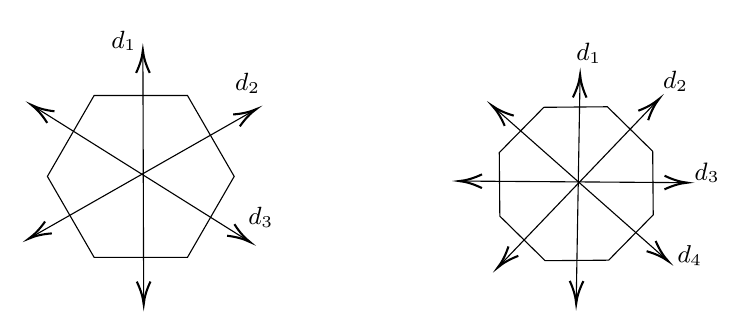
\begin{tikzpicture}[x=0.75pt,y=0.75pt,yscale=-1,xscale=1]
		%uncomment if require: \path (0,300); %set diagram left start at 0, and has height of 300
		
		%Shape: Regular Polygon [id:dp38272018055122115] 
		\draw   (229,100) -- (206.5,138.97) -- (161.5,138.97) -- (139,100) -- (161.5,61.03) -- (206.5,61.03) -- cycle ;
		%Shape: Regular Polygon [id:dp03643618608702448] 
		\draw   (430.63,87.9) -- (430.89,118.52) -- (409.42,140.35) -- (378.81,140.6) -- (356.98,119.14) -- (356.72,88.52) -- (378.19,66.7) -- (408.8,66.44) -- cycle ;
		%Straight Lines [id:da42417542410569764] 
		\draw    (185.39,159.6) -- (185.01,41.2) ;
		\draw [shift={(185,39.2)}, rotate = 89.81] [color={rgb, 255:red, 0; green, 0; blue, 0 }  ][line width=0.75]    (10.93,-3.29) .. controls (6.95,-1.4) and (3.31,-0.3) .. (0,0) .. controls (3.31,0.3) and (6.95,1.4) .. (10.93,3.29)   ;
		\draw [shift={(185.4,161.6)}, rotate = 269.81] [color={rgb, 255:red, 0; green, 0; blue, 0 }  ][line width=0.75]    (10.93,-3.29) .. controls (6.95,-1.4) and (3.31,-0.3) .. (0,0) .. controls (3.31,0.3) and (6.95,1.4) .. (10.93,3.29)   ;
		%Straight Lines [id:da8675028417491909] 
		\draw    (131.74,129.01) -- (237.86,68.59) ;
		\draw [shift={(239.6,67.6)}, rotate = 150.35] [color={rgb, 255:red, 0; green, 0; blue, 0 }  ][line width=0.75]    (10.93,-3.29) .. controls (6.95,-1.4) and (3.31,-0.3) .. (0,0) .. controls (3.31,0.3) and (6.95,1.4) .. (10.93,3.29)   ;
		\draw [shift={(130,130)}, rotate = 330.35] [color={rgb, 255:red, 0; green, 0; blue, 0 }  ][line width=0.75]    (10.93,-3.29) .. controls (6.95,-1.4) and (3.31,-0.3) .. (0,0) .. controls (3.31,0.3) and (6.95,1.4) .. (10.93,3.29)   ;
		%Straight Lines [id:da30906746309807165] 
		\draw    (133.09,66.66) -- (234.91,130.54) ;
		\draw [shift={(236.6,131.6)}, rotate = 212.1] [color={rgb, 255:red, 0; green, 0; blue, 0 }  ][line width=0.75]    (10.93,-3.29) .. controls (6.95,-1.4) and (3.31,-0.3) .. (0,0) .. controls (3.31,0.3) and (6.95,1.4) .. (10.93,3.29)   ;
		\draw [shift={(131.4,65.6)}, rotate = 32.1] [color={rgb, 255:red, 0; green, 0; blue, 0 }  ][line width=0.75]    (10.93,-3.29) .. controls (6.95,-1.4) and (3.31,-0.3) .. (0,0) .. controls (3.31,0.3) and (6.95,1.4) .. (10.93,3.29)   ;
		%Straight Lines [id:da65453798610991] 
		\draw    (393.8,159.32) -- (395.63,53.03) ;
		\draw [shift={(395.66,51.03)}, rotate = 90.98] [color={rgb, 255:red, 0; green, 0; blue, 0 }  ][line width=0.75]    (10.93,-3.29) .. controls (6.95,-1.4) and (3.31,-0.3) .. (0,0) .. controls (3.31,0.3) and (6.95,1.4) .. (10.93,3.29)   ;
		\draw [shift={(393.77,161.32)}, rotate = 270.98] [color={rgb, 255:red, 0; green, 0; blue, 0 }  ][line width=0.75]    (10.93,-3.29) .. controls (6.95,-1.4) and (3.31,-0.3) .. (0,0) .. controls (3.31,0.3) and (6.95,1.4) .. (10.93,3.29)   ;
		%Straight Lines [id:da5174940913781368] 
		\draw    (357.35,142.45) -- (432.26,64.18) ;
		\draw [shift={(433.64,62.73)}, rotate = 133.74] [color={rgb, 255:red, 0; green, 0; blue, 0 }  ][line width=0.75]    (10.93,-3.29) .. controls (6.95,-1.4) and (3.31,-0.3) .. (0,0) .. controls (3.31,0.3) and (6.95,1.4) .. (10.93,3.29)   ;
		\draw [shift={(355.97,143.9)}, rotate = 313.74] [color={rgb, 255:red, 0; green, 0; blue, 0 }  ][line width=0.75]    (10.93,-3.29) .. controls (6.95,-1.4) and (3.31,-0.3) .. (0,0) .. controls (3.31,0.3) and (6.95,1.4) .. (10.93,3.29)   ;
		%Straight Lines [id:da7207208027265464] 
		\draw    (339.43,102.24) -- (445.25,103) ;
		\draw [shift={(447.25,103.02)}, rotate = 180.41] [color={rgb, 255:red, 0; green, 0; blue, 0 }  ][line width=0.75]    (10.93,-3.29) .. controls (6.95,-1.4) and (3.31,-0.3) .. (0,0) .. controls (3.31,0.3) and (6.95,1.4) .. (10.93,3.29)   ;
		\draw [shift={(337.43,102.23)}, rotate = 0.41] [color={rgb, 255:red, 0; green, 0; blue, 0 }  ][line width=0.75]    (10.93,-3.29) .. controls (6.95,-1.4) and (3.31,-0.3) .. (0,0) .. controls (3.31,0.3) and (6.95,1.4) .. (10.93,3.29)   ;
		%Straight Lines [id:da7287534383817258] 
		\draw    (354.82,67.27) -- (436.57,139.47) ;
		\draw [shift={(438.07,140.8)}, rotate = 221.45] [color={rgb, 255:red, 0; green, 0; blue, 0 }  ][line width=0.75]    (10.93,-3.29) .. controls (6.95,-1.4) and (3.31,-0.3) .. (0,0) .. controls (3.31,0.3) and (6.95,1.4) .. (10.93,3.29)   ;
		\draw [shift={(353.32,65.94)}, rotate = 41.45] [color={rgb, 255:red, 0; green, 0; blue, 0 }  ][line width=0.75]    (10.93,-3.29) .. controls (6.95,-1.4) and (3.31,-0.3) .. (0,0) .. controls (3.31,0.3) and (6.95,1.4) .. (10.93,3.29)   ;
		
		% Text Node
		\draw (168.6,28.6) node [anchor=north west][inner sep=0.75pt]  [font=\small]  {$d_{1}$};
		% Text Node
		\draw (228.2,49) node [anchor=north west][inner sep=0.75pt]  [font=\small]  {$d_{2}$};
		% Text Node
		\draw (234.6,113.6) node [anchor=north west][inner sep=0.75pt]  [font=\small]  {$d_{3}$};
		% Text Node
		\draw (441.48,131.94) node [anchor=north west][inner sep=0.75pt]  [font=\small,rotate=-1.57]  {$d_{4}$};
		% Text Node
		\draw (392.55,34.66) node [anchor=north west][inner sep=0.75pt]  [font=\small,rotate=-359.55]  {$d_{1}$};
		% Text Node
		\draw (434.39,48.18) node [anchor=north west][inner sep=0.75pt]  [font=\small,rotate=-359.8]  {$d_{2}$};
		% Text Node
		\draw (449.46,92.26) node [anchor=north west][inner sep=0.75pt]  [font=\small,rotate=-359.03]  {$d_{3}$};
		
		
	\end{tikzpicture}
\end{figure}
	However, for these tiles with more number of sides, if we enable the rotation of flipping of tiles, then the tile-tile interaction graph gets very crowded very fast. So we want to utilize as much of the symmetry as possible.
	
	
	\subsubsection{Utilizing the Symmetries}
	
	For now, consider we have three types of glue $ G = \{g_1,g_2,g_3\} $, and only one tile  that has the glue profile $  g_1g_2g_3g_1  $, denoted by $ t $. Furthermore, consider the following glue-glue interaction matrix
	\[ s = \begin{pmatrix}
		0 & 0 & 1 \\
		0 & 1 & 1 \\
		1 & 1 & 1 
	\end{pmatrix}. \]
	 We also enable rotations of the tile, but we do not use the same naming conventions as used above, but instead we fix the permutation $ \sigma $ that rotates the square 90 degrees \textit{counter clockwise}. Thus the set of tiles will be
	\[ T = \{ \sigma^0 t, \sigma^1 t, \sigma^2 t, \sigma^3 t \}. \]
	\begin{figure}[h!]
	\centering
	
	
	\tikzset{every picture/.style={line width=0.75pt}} %set default line width to 0.75pt        
	
	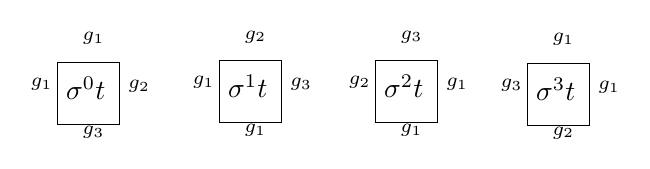
\begin{tikzpicture}[x=0.75pt,y=0.75pt,yscale=-1,xscale=1]
		%uncomment if require: \path (0,300); %set diagram left start at 0, and has height of 300
		
		%Shape: Square [id:dp9064068834085001] 
		\draw   (109.2,72.2) -- (139.2,72.2) -- (139.2,102.2) -- (109.2,102.2) -- cycle ;
		%Shape: Square [id:dp43325954116246435] 
		\draw   (187.2,71.4) -- (217.2,71.4) -- (217.2,101.4) -- (187.2,101.4) -- cycle ;
		%Shape: Square [id:dp6235327177004354] 
		\draw   (262.4,71.4) -- (292.4,71.4) -- (292.4,101.4) -- (262.4,101.4) -- cycle ;
		%Shape: Square [id:dp07042046594573603] 
		\draw   (335.6,72.6) -- (365.6,72.6) -- (365.6,102.6) -- (335.6,102.6) -- cycle ;
		
		% Text Node
		\draw (120.2,56.6) node [anchor=north west][inner sep=0.75pt]  [font=\scriptsize]  {$g_{1}$};
		% Text Node
		\draw (142.2,79.6) node [anchor=north west][inner sep=0.75pt]  [font=\scriptsize]  {$g_{2}$};
		% Text Node
		\draw (120.2,101.6) node [anchor=north west][inner sep=0.75pt]  [font=\scriptsize]  {$g_{3}$};
		% Text Node
		\draw (95.2,78.6) node [anchor=north west][inner sep=0.75pt]  [font=\scriptsize]  {$g_{1}$};
		% Text Node
		\draw (112.2,78) node [anchor=north west][inner sep=0.75pt]    {$\sigma ^{0} t$};
		% Text Node
		\draw (198.2,55.8) node [anchor=north west][inner sep=0.75pt]  [font=\scriptsize]  {$g_{2}$};
		% Text Node
		\draw (220.2,78.8) node [anchor=north west][inner sep=0.75pt]  [font=\scriptsize]  {$g_{3}$};
		% Text Node
		\draw (198.2,100.8) node [anchor=north west][inner sep=0.75pt]  [font=\scriptsize]  {$g_{1}$};
		% Text Node
		\draw (173.2,77.8) node [anchor=north west][inner sep=0.75pt]  [font=\scriptsize]  {$g_{1}$};
		% Text Node
		\draw (190.2,77.2) node [anchor=north west][inner sep=0.75pt]    {$\sigma ^{1} t$};
		% Text Node
		\draw (273.4,55.8) node [anchor=north west][inner sep=0.75pt]  [font=\scriptsize]  {$g_{3}$};
		% Text Node
		\draw (295.4,78.8) node [anchor=north west][inner sep=0.75pt]  [font=\scriptsize]  {$g_{1}$};
		% Text Node
		\draw (273.4,100.8) node [anchor=north west][inner sep=0.75pt]  [font=\scriptsize]  {$g_{1}$};
		% Text Node
		\draw (248.4,77.8) node [anchor=north west][inner sep=0.75pt]  [font=\scriptsize]  {$g_{2}$};
		% Text Node
		\draw (265.4,77.2) node [anchor=north west][inner sep=0.75pt]    {$\sigma ^{2} t$};
		% Text Node
		\draw (346.6,57) node [anchor=north west][inner sep=0.75pt]  [font=\scriptsize]  {$g_{1}$};
		% Text Node
		\draw (368.6,80) node [anchor=north west][inner sep=0.75pt]  [font=\scriptsize]  {$g_{1}$};
		% Text Node
		\draw (346.6,102) node [anchor=north west][inner sep=0.75pt]  [font=\scriptsize]  {$g_{2}$};
		% Text Node
		\draw (321.6,79) node [anchor=north west][inner sep=0.75pt]  [font=\scriptsize]  {$g_{3}$};
		% Text Node
		\draw (338.6,78.4) node [anchor=north west][inner sep=0.75pt]    {$\sigma ^{3} t$};
		
		
	\end{tikzpicture}
\end{figure}
	Then each of the partitions $ N,E,S,W $ are related in a very interesting way. Enumerating the alphabet position in the tile code $ g_1g_2g_3g_1 $ from $ 0 $ to $ 3 $, it is straight forward to construct the equivalence classes for the $ N $ relation. Since $ g_1 $ has appeared in the 0 and 3 positions, then $ [g_1]_N = \{\sigma^0t, \sigma^3t\} $. Similarly, since $ g_2 $ only occupies the 1 position, then $ [g_2]_N =\{ \sigma^1 t\} $, and lastly $ g_3 $ being on the 2 position we have $ [g_3]_N = \{\sigma^2 t\} $. In short
	\[ [g_1]_N = \{ \sigma^0 t, \sigma^3 t \},\quad [g_2]_N = \{\sigma^1t\}, \quad [g_3]_N = \{ \sigma^2t \}. \]
	Furthermore, observe the following relation between $ N,E,S $, and $ W $ directions:
	\[ N = \sigma^0 N, \qquad W = \sigma^1 N, \qquad S = \sigma^2 N, \qquad E = \sigma^3 N, \]
	where one can interpret the multiplications above as just formal symbolic multiplication as there is no group structure present. Then it is easy to see that
	\[ [g]_{\sigma^n N} = \sigma^n [g]_{N}. \]
	So knowing the equivalence classes for $ N $, and knowing how to transform $ N $ to other relations by rotation $ \sigma $, one can easily calculate the other equivalence relations as follows
	\[ [g]_W = \sigma\cdot [g]_N, \qquad [g]_S = \sigma^2\cdot [g]_N, \qquad [g]_E = \sigma^3\cdot [g]_N, \]
	where the multiplication $ \cdot $ should be interpreted as multiplying every element in the set. Using the glue-glue interaction matrix we will get
	\begin{figure}[h!]
	\centering
	
	
	
	\tikzset{every picture/.style={line width=0.75pt}} %set default line width to 0.75pt        
	
	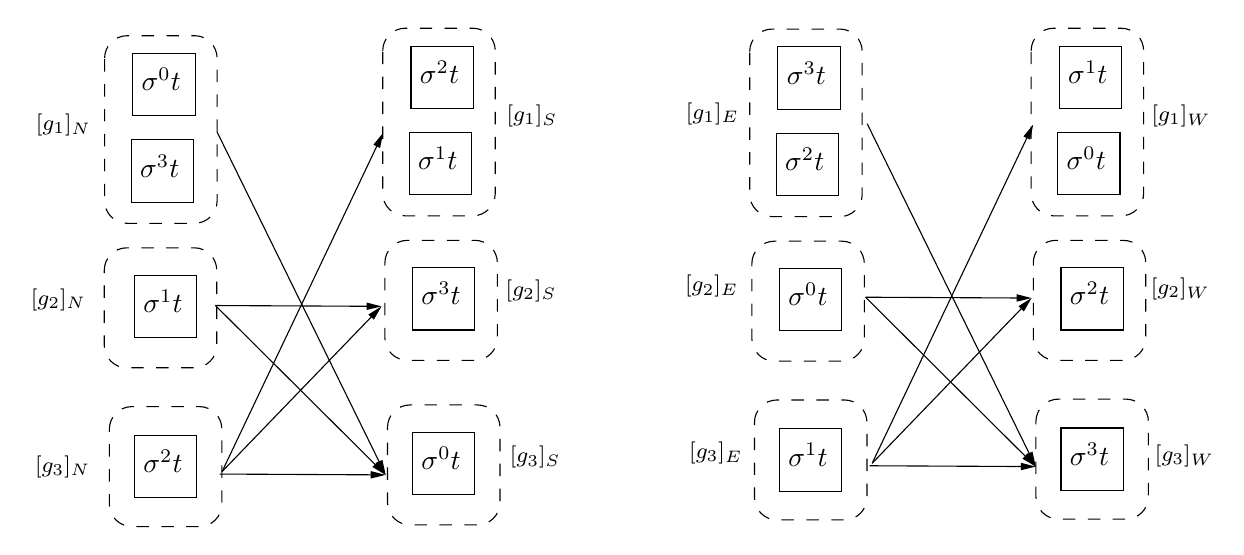
\begin{tikzpicture}[x=0.75pt,y=0.75pt,yscale=-1,xscale=1]
		%uncomment if require: \path (0,300); %set diagram left start at 0, and has height of 300
		
		%Shape: Square [id:dp9064068834085001] 
		\draw   (90.4,31.8) -- (120.4,31.8) -- (120.4,61.8) -- (90.4,61.8) -- cycle ;
		%Shape: Square [id:dp43325954116246435] 
		\draw   (91.2,138.6) -- (121.2,138.6) -- (121.2,168.6) -- (91.2,168.6) -- cycle ;
		%Shape: Square [id:dp6235327177004354] 
		\draw   (91.2,215.8) -- (121.2,215.8) -- (121.2,245.8) -- (91.2,245.8) -- cycle ;
		%Shape: Square [id:dp07042046594573603] 
		\draw   (89.6,73.4) -- (119.6,73.4) -- (119.6,103.4) -- (89.6,103.4) -- cycle ;
		%Rounded Rect [id:dp04567549240458135] 
		\draw  [dash pattern={on 4.5pt off 4.5pt}] (76.8,34.04) .. controls (76.8,28.05) and (81.65,23.2) .. (87.64,23.2) -- (120.16,23.2) .. controls (126.15,23.2) and (131,28.05) .. (131,34.04) -- (131,102.76) .. controls (131,108.75) and (126.15,113.6) .. (120.16,113.6) -- (87.64,113.6) .. controls (81.65,113.6) and (76.8,108.75) .. (76.8,102.76) -- cycle ;
		%Rounded Rect [id:dp14969692621734598] 
		\draw  [dash pattern={on 4.5pt off 4.5pt}] (76.64,136.24) .. controls (76.64,130.25) and (81.49,125.4) .. (87.48,125.4) -- (120,125.4) .. controls (125.99,125.4) and (130.84,130.25) .. (130.84,136.24) -- (130.84,172.36) .. controls (130.84,178.35) and (125.99,183.2) .. (120,183.2) -- (87.48,183.2) .. controls (81.49,183.2) and (76.64,178.35) .. (76.64,172.36) -- cycle ;
		%Rounded Rect [id:dp5835633898501008] 
		\draw  [dash pattern={on 4.5pt off 4.5pt}] (79.1,212.74) .. controls (79.1,206.75) and (83.95,201.9) .. (89.94,201.9) -- (122.46,201.9) .. controls (128.45,201.9) and (133.3,206.75) .. (133.3,212.74) -- (133.3,248.86) .. controls (133.3,254.85) and (128.45,259.7) .. (122.46,259.7) -- (89.94,259.7) .. controls (83.95,259.7) and (79.1,254.85) .. (79.1,248.86) -- cycle ;
		%Shape: Square [id:dp12847607358099766] 
		\draw   (224.4,28.2) -- (254.4,28.2) -- (254.4,58.2) -- (224.4,58.2) -- cycle ;
		%Shape: Square [id:dp9789211274161613] 
		\draw   (225.2,135) -- (255.2,135) -- (255.2,165) -- (225.2,165) -- cycle ;
		%Shape: Square [id:dp8548913004980881] 
		\draw   (225.2,214.2) -- (255.2,214.2) -- (255.2,244.2) -- (225.2,244.2) -- cycle ;
		%Shape: Square [id:dp556021413809052] 
		\draw   (223.6,69.8) -- (253.6,69.8) -- (253.6,99.8) -- (223.6,99.8) -- cycle ;
		%Rounded Rect [id:dp23096578553301506] 
		\draw  [dash pattern={on 4.5pt off 4.5pt}] (210.8,30.44) .. controls (210.8,24.45) and (215.65,19.6) .. (221.64,19.6) -- (254.16,19.6) .. controls (260.15,19.6) and (265,24.45) .. (265,30.44) -- (265,99.16) .. controls (265,105.15) and (260.15,110) .. (254.16,110) -- (221.64,110) .. controls (215.65,110) and (210.8,105.15) .. (210.8,99.16) -- cycle ;
		%Rounded Rect [id:dp006100142826457211] 
		\draw  [dash pattern={on 4.5pt off 4.5pt}] (211.84,132.64) .. controls (211.84,126.65) and (216.69,121.8) .. (222.68,121.8) -- (255.2,121.8) .. controls (261.19,121.8) and (266.04,126.65) .. (266.04,132.64) -- (266.04,168.76) .. controls (266.04,174.75) and (261.19,179.6) .. (255.2,179.6) -- (222.68,179.6) .. controls (216.69,179.6) and (211.84,174.75) .. (211.84,168.76) -- cycle ;
		%Rounded Rect [id:dp8021063767257534] 
		\draw  [dash pattern={on 4.5pt off 4.5pt}] (213.1,211.94) .. controls (213.1,205.95) and (217.95,201.1) .. (223.94,201.1) -- (256.46,201.1) .. controls (262.45,201.1) and (267.3,205.95) .. (267.3,211.94) -- (267.3,248.06) .. controls (267.3,254.05) and (262.45,258.9) .. (256.46,258.9) -- (223.94,258.9) .. controls (217.95,258.9) and (213.1,254.05) .. (213.1,248.06) -- cycle ;
		%Shape: Square [id:dp0390861871153686] 
		\draw   (401.2,28.6) -- (431.2,28.6) -- (431.2,58.6) -- (401.2,58.6) -- cycle ;
		%Shape: Square [id:dp2794369563185318] 
		\draw   (402,135.4) -- (432,135.4) -- (432,165.4) -- (402,165.4) -- cycle ;
		%Shape: Square [id:dp8317205428086728] 
		\draw   (402,212.6) -- (432,212.6) -- (432,242.6) -- (402,242.6) -- cycle ;
		%Shape: Square [id:dp17113062398485046] 
		\draw   (400.4,70.2) -- (430.4,70.2) -- (430.4,100.2) -- (400.4,100.2) -- cycle ;
		%Rounded Rect [id:dp6452244939455726] 
		\draw  [dash pattern={on 4.5pt off 4.5pt}] (387.6,30.84) .. controls (387.6,24.85) and (392.45,20) .. (398.44,20) -- (430.96,20) .. controls (436.95,20) and (441.8,24.85) .. (441.8,30.84) -- (441.8,99.56) .. controls (441.8,105.55) and (436.95,110.4) .. (430.96,110.4) -- (398.44,110.4) .. controls (392.45,110.4) and (387.6,105.55) .. (387.6,99.56) -- cycle ;
		%Rounded Rect [id:dp7833844751184817] 
		\draw  [dash pattern={on 4.5pt off 4.5pt}] (388.64,133.04) .. controls (388.64,127.05) and (393.49,122.2) .. (399.48,122.2) -- (432,122.2) .. controls (437.99,122.2) and (442.84,127.05) .. (442.84,133.04) -- (442.84,169.16) .. controls (442.84,175.15) and (437.99,180) .. (432,180) -- (399.48,180) .. controls (393.49,180) and (388.64,175.15) .. (388.64,169.16) -- cycle ;
		%Rounded Rect [id:dp6296850203465514] 
		\draw  [dash pattern={on 4.5pt off 4.5pt}] (389.9,209.54) .. controls (389.9,203.55) and (394.75,198.7) .. (400.74,198.7) -- (433.26,198.7) .. controls (439.25,198.7) and (444.1,203.55) .. (444.1,209.54) -- (444.1,245.66) .. controls (444.1,251.65) and (439.25,256.5) .. (433.26,256.5) -- (400.74,256.5) .. controls (394.75,256.5) and (389.9,251.65) .. (389.9,245.66) -- cycle ;
		%Shape: Square [id:dp1663169666422517] 
		\draw   (536.8,28.2) -- (566.8,28.2) -- (566.8,58.2) -- (536.8,58.2) -- cycle ;
		%Shape: Square [id:dp9758574935521903] 
		\draw   (537.6,135) -- (567.6,135) -- (567.6,165) -- (537.6,165) -- cycle ;
		%Shape: Square [id:dp6867963655749864] 
		\draw   (537.6,212.2) -- (567.6,212.2) -- (567.6,242.2) -- (537.6,242.2) -- cycle ;
		%Shape: Square [id:dp3685257473693341] 
		\draw   (536,69.8) -- (566,69.8) -- (566,99.8) -- (536,99.8) -- cycle ;
		%Rounded Rect [id:dp5445918417179938] 
		\draw  [dash pattern={on 4.5pt off 4.5pt}] (523.2,30.44) .. controls (523.2,24.45) and (528.05,19.6) .. (534.04,19.6) -- (566.56,19.6) .. controls (572.55,19.6) and (577.4,24.45) .. (577.4,30.44) -- (577.4,99.16) .. controls (577.4,105.15) and (572.55,110) .. (566.56,110) -- (534.04,110) .. controls (528.05,110) and (523.2,105.15) .. (523.2,99.16) -- cycle ;
		%Rounded Rect [id:dp2657715758325272] 
		\draw  [dash pattern={on 4.5pt off 4.5pt}] (524.24,132.64) .. controls (524.24,126.65) and (529.09,121.8) .. (535.08,121.8) -- (567.6,121.8) .. controls (573.59,121.8) and (578.44,126.65) .. (578.44,132.64) -- (578.44,168.76) .. controls (578.44,174.75) and (573.59,179.6) .. (567.6,179.6) -- (535.08,179.6) .. controls (529.09,179.6) and (524.24,174.75) .. (524.24,168.76) -- cycle ;
		%Rounded Rect [id:dp45090338404001107] 
		\draw  [dash pattern={on 4.5pt off 4.5pt}] (525.5,209.14) .. controls (525.5,203.15) and (530.35,198.3) .. (536.34,198.3) -- (568.86,198.3) .. controls (574.85,198.3) and (579.7,203.15) .. (579.7,209.14) -- (579.7,245.26) .. controls (579.7,251.25) and (574.85,256.1) .. (568.86,256.1) -- (536.34,256.1) .. controls (530.35,256.1) and (525.5,251.25) .. (525.5,245.26) -- cycle ;
		%Straight Lines [id:da5768247022482709] 
		\draw    (131,69.6) -- (211.32,233.01) ;
		\draw [shift={(212.2,234.8)}, rotate = 243.82] [fill={rgb, 255:red, 0; green, 0; blue, 0 }  ][line width=0.08]  [draw opacity=0] (7.2,-1.8) -- (0,0) -- (7.2,1.8) -- cycle    ;
		%Straight Lines [id:da9461999197171234] 
		\draw    (130.2,153.2) -- (208.2,153.59) ;
		\draw [shift={(210.2,153.6)}, rotate = 180.29] [fill={rgb, 255:red, 0; green, 0; blue, 0 }  ][line width=0.08]  [draw opacity=0] (7.2,-1.8) -- (0,0) -- (7.2,1.8) -- cycle    ;
		%Straight Lines [id:da029865164366322472] 
		\draw    (133.4,233.2) -- (210.14,71.81) ;
		\draw [shift={(211,70)}, rotate = 115.43] [fill={rgb, 255:red, 0; green, 0; blue, 0 }  ][line width=0.08]  [draw opacity=0] (7.2,-1.8) -- (0,0) -- (7.2,1.8) -- cycle    ;
		%Straight Lines [id:da7625101249140692] 
		\draw    (130.2,153.2) -- (210.78,233.39) ;
		\draw [shift={(212.2,234.8)}, rotate = 224.86] [fill={rgb, 255:red, 0; green, 0; blue, 0 }  ][line width=0.08]  [draw opacity=0] (7.2,-1.8) -- (0,0) -- (7.2,1.8) -- cycle    ;
		%Straight Lines [id:da5219613321995814] 
		\draw    (132.2,234.4) -- (210.2,234.79) ;
		\draw [shift={(212.2,234.8)}, rotate = 180.29] [fill={rgb, 255:red, 0; green, 0; blue, 0 }  ][line width=0.08]  [draw opacity=0] (7.2,-1.8) -- (0,0) -- (7.2,1.8) -- cycle    ;
		%Straight Lines [id:da41273784931961155] 
		\draw    (133.4,233.2) -- (208.81,155.04) ;
		\draw [shift={(210.2,153.6)}, rotate = 133.97] [fill={rgb, 255:red, 0; green, 0; blue, 0 }  ][line width=0.08]  [draw opacity=0] (7.2,-1.8) -- (0,0) -- (7.2,1.8) -- cycle    ;
		%Straight Lines [id:da5329225043284657] 
		\draw    (444.2,65.6) -- (524.52,229.01) ;
		\draw [shift={(525.4,230.8)}, rotate = 243.82] [fill={rgb, 255:red, 0; green, 0; blue, 0 }  ][line width=0.08]  [draw opacity=0] (7.2,-1.8) -- (0,0) -- (7.2,1.8) -- cycle    ;
		%Straight Lines [id:da40090490608233387] 
		\draw    (443.4,149.2) -- (521.4,149.59) ;
		\draw [shift={(523.4,149.6)}, rotate = 180.29] [fill={rgb, 255:red, 0; green, 0; blue, 0 }  ][line width=0.08]  [draw opacity=0] (7.2,-1.8) -- (0,0) -- (7.2,1.8) -- cycle    ;
		%Straight Lines [id:da622218065673155] 
		\draw    (446.6,229.2) -- (523.34,67.81) ;
		\draw [shift={(524.2,66)}, rotate = 115.43] [fill={rgb, 255:red, 0; green, 0; blue, 0 }  ][line width=0.08]  [draw opacity=0] (7.2,-1.8) -- (0,0) -- (7.2,1.8) -- cycle    ;
		%Straight Lines [id:da5014854043424674] 
		\draw    (443.4,149.2) -- (523.98,229.39) ;
		\draw [shift={(525.4,230.8)}, rotate = 224.86] [fill={rgb, 255:red, 0; green, 0; blue, 0 }  ][line width=0.08]  [draw opacity=0] (7.2,-1.8) -- (0,0) -- (7.2,1.8) -- cycle    ;
		%Straight Lines [id:da5997955233993555] 
		\draw    (445.4,230.4) -- (523.4,230.79) ;
		\draw [shift={(525.4,230.8)}, rotate = 180.29] [fill={rgb, 255:red, 0; green, 0; blue, 0 }  ][line width=0.08]  [draw opacity=0] (7.2,-1.8) -- (0,0) -- (7.2,1.8) -- cycle    ;
		%Straight Lines [id:da2510203540727617] 
		\draw    (446.6,229.2) -- (522.01,151.04) ;
		\draw [shift={(523.4,149.6)}, rotate = 133.97] [fill={rgb, 255:red, 0; green, 0; blue, 0 }  ][line width=0.08]  [draw opacity=0] (7.2,-1.8) -- (0,0) -- (7.2,1.8) -- cycle    ;
		
		% Text Node
		\draw (93.4,37.6) node [anchor=north west][inner sep=0.75pt]    {$\sigma ^{0} t$};
		% Text Node
		\draw (94.2,144.4) node [anchor=north west][inner sep=0.75pt]    {$\sigma ^{1} t$};
		% Text Node
		\draw (94.2,221.6) node [anchor=north west][inner sep=0.75pt]    {$\sigma ^{2} t$};
		% Text Node
		\draw (92.6,79.2) node [anchor=north west][inner sep=0.75pt]    {$\sigma ^{3} t$};
		% Text Node
		\draw (227.4,34) node [anchor=north west][inner sep=0.75pt]    {$\sigma ^{2} t$};
		% Text Node
		\draw (228.2,140.8) node [anchor=north west][inner sep=0.75pt]    {$\sigma ^{3} t$};
		% Text Node
		\draw (228.2,220) node [anchor=north west][inner sep=0.75pt]    {$\sigma ^{0} t$};
		% Text Node
		\draw (226.6,75.6) node [anchor=north west][inner sep=0.75pt]    {$\sigma ^{1} t$};
		% Text Node
		\draw (404.2,34.4) node [anchor=north west][inner sep=0.75pt]    {$\sigma ^{3} t$};
		% Text Node
		\draw (405,141.2) node [anchor=north west][inner sep=0.75pt]    {$\sigma ^{0} t$};
		% Text Node
		\draw (405,218.4) node [anchor=north west][inner sep=0.75pt]    {$\sigma ^{1} t$};
		% Text Node
		\draw (403.4,76) node [anchor=north west][inner sep=0.75pt]    {$\sigma ^{2} t$};
		% Text Node
		\draw (539.8,34) node [anchor=north west][inner sep=0.75pt]    {$\sigma ^{1} t$};
		% Text Node
		\draw (540.6,140.8) node [anchor=north west][inner sep=0.75pt]    {$\sigma ^{2} t$};
		% Text Node
		\draw (540.6,218) node [anchor=north west][inner sep=0.75pt]    {$\sigma ^{3} t$};
		% Text Node
		\draw (539,75.6) node [anchor=north west][inner sep=0.75pt]    {$\sigma ^{0} t$};
		% Text Node
		\draw (42.4,59.8) node [anchor=north west][inner sep=0.75pt]  [font=\footnotesize]  {$[ g_{1}]_{N}$};
		% Text Node
		\draw (40,143.8) node [anchor=north west][inner sep=0.75pt]  [font=\footnotesize]  {$[ g_{2}]_{N}$};
		% Text Node
		\draw (42,224.2) node [anchor=north west][inner sep=0.75pt]  [font=\footnotesize]  {$[ g_{3}]_{N}$};
		% Text Node
		\draw (269.2,55.4) node [anchor=north west][inner sep=0.75pt]  [font=\footnotesize]  {$[ g_{1}]_{S}$};
		% Text Node
		\draw (268.8,139.4) node [anchor=north west][inner sep=0.75pt]  [font=\footnotesize]  {$[ g_{2}]_{S}$};
		% Text Node
		\draw (270.8,219.8) node [anchor=north west][inner sep=0.75pt]  [font=\footnotesize]  {$[ g_{3}]_{S}$};
		% Text Node
		\draw (355.6,54.2) node [anchor=north west][inner sep=0.75pt]  [font=\footnotesize]  {$[ g_{1}]_{E}$};
		% Text Node
		\draw (355.2,137.4) node [anchor=north west][inner sep=0.75pt]  [font=\footnotesize]  {$[ g_{2}]_{E}$};
		% Text Node
		\draw (357.2,217.8) node [anchor=north west][inner sep=0.75pt]  [font=\footnotesize]  {$[ g_{3}]_{E}$};
		% Text Node
		\draw (580,55.4) node [anchor=north west][inner sep=0.75pt]  [font=\footnotesize]  {$[ g_{1}]_{W}$};
		% Text Node
		\draw (579.6,138.6) node [anchor=north west][inner sep=0.75pt]  [font=\footnotesize]  {$[ g_{2}]_{W}$};
		% Text Node
		\draw (581.6,219) node [anchor=north west][inner sep=0.75pt]  [font=\footnotesize]  {$[ g_{3}]_{W}$};
		
		
	\end{tikzpicture}
\end{figure}
 	\FloatBarrier
 	
 	
 	\subsubsection{A Complete Worked Example}
 	
 	To demonstrate the capabilities of this approach, here we are presenting a complete worked example where we have 4 type of glue $ g = \{g_1,g_2,g_3,g_4\} $, and 5 types of tiles
 	\[ T = \{ \tile{t_1},\tile{t_2},\tile{t_3},\tile{t_4},\tile{t_5} \}, \]
 	where
 	\[ t_1=g_3g_1g_4g_2,\quad t_2=g_2g_2g_3g_1,\quad t_3=g_4g_1g_4g_3,\quad t_4=g_1g_3g_2g_2,\quad t_5=g_2g_4g_1g_3. \]
 	Also, assume that the following glue-glue interaction is given:
 	\[ 
 	s = \begin{pmatrix}
 		1 & 1 & 0 & 1\\
 		1 & 1 & 1 & 0\\
 		0 & 1 & 0 & 1\\
 		1 & 0 & 1 & 0
 	\end{pmatrix}.
 	 \]
 	Also assume that we allow rotations. Let $ \sigma $ denote the counterclockwise rotation, i.e. $ \sigma t_1 = g_1g_4g_2g_3 $, and etc. Now it is easy to build the equivalence classes corresponding to the $ N $ relation:
 	\[ [g_1]_N = \{ \sigma^1t_1, \sigma^3t_2, \sigma^1t_3, \sigma^0t_4, \sigma^2t_5 \}, \]
 	\[ [g_2]_N = \{ \sigma^3t_1, \sigma^0t_2, \sigma^1t_2, \sigma^2t_4, \sigma^3t_4, \sigma^0t_5\}, \]
 	\[ [g_3]_N = \{ \sigma^0t_1, \sigma^2t_2, \sigma^3t_3, \sigma^1t_4, \sigma^3t_5 \}, \]
 	\[ [g_4]_N = \{ \sigma^2t_1, \sigma^0t_3, \sigma^2t_3, \sigma^1t_5 \}. \]
 	Using the laws discussed above, it is easy to calculate the equivalence classes for other relations as well. For $ W $:
 	\[ [g_1]_W = \sigma [g_1]_N = \{ \sigma^2t_1, \sigma^0t_2, \sigma^2t_3, \sigma^1t_4, \sigma^3t_5 \}, \]
 	\[ [g_2]_W = \{ \sigma^0t_1, \sigma^1t_2, \sigma^2t_2, \sigma^3t_4, \sigma^0t_4, \sigma^1t_5\}, \]
 	\[ [g_3]_W  = \{ \sigma^1t_1, \sigma^3t_2, \sigma^0t_3, \sigma^2t_4, \sigma^0t_5 \},  \]
 	\[ [g_4]_W = \{ \sigma^3t_1, \sigma^1t_3, \sigma^3t_3, \sigma^2t_5 \}, \]
 	for $ S $:
 	\[ [g_1]_S = \{ \sigma^3t_1, \sigma^1t_2, \sigma^3t_3, \sigma^2t_4, \sigma^0t_5 \}, \]
 	\[ [g_2]_S = \{ \sigma^1t_1, \sigma^2t_2, \sigma^3t_2, \sigma^0t_4, \sigma^1t_4, \sigma^2t_5\}, \]
 	\[ [g_3]_S  = \{ \sigma^2t_1, \sigma^0t_2, \sigma^1t_3, \sigma^3t_4, \sigma^1t_5 \},  \]
 	\[ [g_4]_S = \{ \sigma^0t_1, \sigma^2t_3, \sigma^0t_3, \sigma^3t_5 \}, \]
 	for $ E $:
 	\[ [g_1]_E = \{ \sigma^0t_1, \sigma^2t_2, \sigma^0t_3, \sigma^3t_4, \sigma^1t_5 \}, \]
 	\[ [g_2]_E = \{ \sigma^2t_1, \sigma^3t_2, \sigma^0t_2, \sigma^1t_4, \sigma^2t_4, \sigma^3t_5\}, \]
 	\[ [g_3]_E  = \{ \sigma^3t_1, \sigma^1t_2, \sigma^2t_3, \sigma^0t_4, \sigma^2t_5 \},  \]
 	\[ [g_4]_E = \{ \sigma^1t_1, \sigma^3t_3, \sigma^1t_3, \sigma^0t_5 \}, \]
 	and so on. Using the glue-glue interaction matrix, the connection between partitions will be as follows
 	\begin{figure}[h!]
	\centering
	
	
	\tikzset{every picture/.style={line width=0.75pt}} %set default line width to 0.75pt        
	
	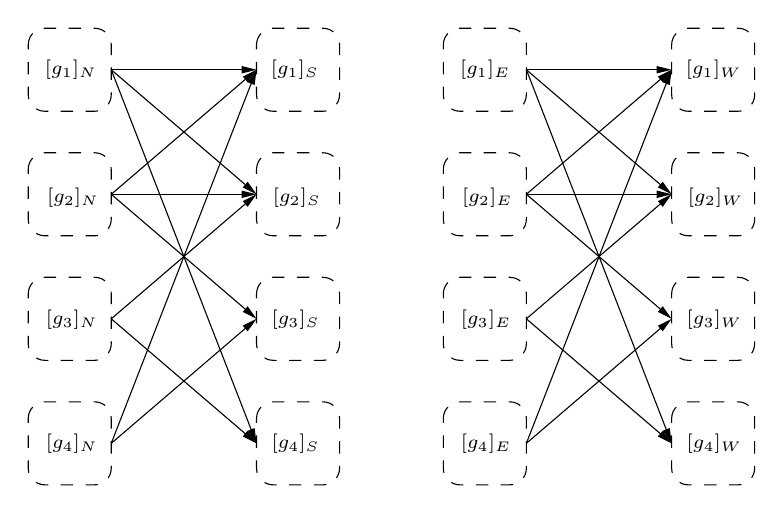
\begin{tikzpicture}[x=0.75pt,y=0.75pt,yscale=-1,xscale=1]
		%uncomment if require: \path (0,300); %set diagram left start at 0, and has height of 300
		
		%Rounded Rect [id:dp5377426226557697] 
		\draw  [dash pattern={on 4.5pt off 4.5pt}] (80,28) .. controls (80,23.58) and (83.58,20) .. (88,20) -- (112,20) .. controls (116.42,20) and (120,23.58) .. (120,28) -- (120,52) .. controls (120,56.42) and (116.42,60) .. (112,60) -- (88,60) .. controls (83.58,60) and (80,56.42) .. (80,52) -- cycle ;
		%Rounded Rect [id:dp20309017644002758] 
		\draw  [dash pattern={on 4.5pt off 4.5pt}] (80,88) .. controls (80,83.58) and (83.58,80) .. (88,80) -- (112,80) .. controls (116.42,80) and (120,83.58) .. (120,88) -- (120,112) .. controls (120,116.42) and (116.42,120) .. (112,120) -- (88,120) .. controls (83.58,120) and (80,116.42) .. (80,112) -- cycle ;
		%Rounded Rect [id:dp6052151502300683] 
		\draw  [dash pattern={on 4.5pt off 4.5pt}] (80,148) .. controls (80,143.58) and (83.58,140) .. (88,140) -- (112,140) .. controls (116.42,140) and (120,143.58) .. (120,148) -- (120,172) .. controls (120,176.42) and (116.42,180) .. (112,180) -- (88,180) .. controls (83.58,180) and (80,176.42) .. (80,172) -- cycle ;
		%Rounded Rect [id:dp36611762003414694] 
		\draw  [dash pattern={on 4.5pt off 4.5pt}] (80,208) .. controls (80,203.58) and (83.58,200) .. (88,200) -- (112,200) .. controls (116.42,200) and (120,203.58) .. (120,208) -- (120,232) .. controls (120,236.42) and (116.42,240) .. (112,240) -- (88,240) .. controls (83.58,240) and (80,236.42) .. (80,232) -- cycle ;
		%Rounded Rect [id:dp5757820056329745] 
		\draw  [dash pattern={on 4.5pt off 4.5pt}] (190,28) .. controls (190,23.58) and (193.58,20) .. (198,20) -- (222,20) .. controls (226.42,20) and (230,23.58) .. (230,28) -- (230,52) .. controls (230,56.42) and (226.42,60) .. (222,60) -- (198,60) .. controls (193.58,60) and (190,56.42) .. (190,52) -- cycle ;
		%Rounded Rect [id:dp6172429033691823] 
		\draw  [dash pattern={on 4.5pt off 4.5pt}] (190,88) .. controls (190,83.58) and (193.58,80) .. (198,80) -- (222,80) .. controls (226.42,80) and (230,83.58) .. (230,88) -- (230,112) .. controls (230,116.42) and (226.42,120) .. (222,120) -- (198,120) .. controls (193.58,120) and (190,116.42) .. (190,112) -- cycle ;
		%Rounded Rect [id:dp19794669737432335] 
		\draw  [dash pattern={on 4.5pt off 4.5pt}] (190,148) .. controls (190,143.58) and (193.58,140) .. (198,140) -- (222,140) .. controls (226.42,140) and (230,143.58) .. (230,148) -- (230,172) .. controls (230,176.42) and (226.42,180) .. (222,180) -- (198,180) .. controls (193.58,180) and (190,176.42) .. (190,172) -- cycle ;
		%Rounded Rect [id:dp06336304386760261] 
		\draw  [dash pattern={on 4.5pt off 4.5pt}] (190,208) .. controls (190,203.58) and (193.58,200) .. (198,200) -- (222,200) .. controls (226.42,200) and (230,203.58) .. (230,208) -- (230,232) .. controls (230,236.42) and (226.42,240) .. (222,240) -- (198,240) .. controls (193.58,240) and (190,236.42) .. (190,232) -- cycle ;
		%Straight Lines [id:da7946178085798109] 
		\draw    (120,40) -- (188,40) ;
		\draw [shift={(190,40)}, rotate = 180] [fill={rgb, 255:red, 0; green, 0; blue, 0 }  ][line width=0.08]  [draw opacity=0] (7.2,-1.8) -- (0,0) -- (7.2,1.8) -- cycle    ;
		%Straight Lines [id:da2734482545518069] 
		\draw    (120,40) -- (188.48,98.7) ;
		\draw [shift={(190,100)}, rotate = 220.6] [fill={rgb, 255:red, 0; green, 0; blue, 0 }  ][line width=0.08]  [draw opacity=0] (7.2,-1.8) -- (0,0) -- (7.2,1.8) -- cycle    ;
		%Straight Lines [id:da7832316713577047] 
		\draw    (120,40) -- (189.28,218.14) ;
		\draw [shift={(190,220)}, rotate = 248.75] [fill={rgb, 255:red, 0; green, 0; blue, 0 }  ][line width=0.08]  [draw opacity=0] (7.2,-1.8) -- (0,0) -- (7.2,1.8) -- cycle    ;
		%Straight Lines [id:da4517238625421285] 
		\draw    (120,100) -- (188.48,41.3) ;
		\draw [shift={(190,40)}, rotate = 139.4] [fill={rgb, 255:red, 0; green, 0; blue, 0 }  ][line width=0.08]  [draw opacity=0] (7.2,-1.8) -- (0,0) -- (7.2,1.8) -- cycle    ;
		%Straight Lines [id:da31866394748760274] 
		\draw    (120,100) -- (188,100) ;
		\draw [shift={(190,100)}, rotate = 180] [fill={rgb, 255:red, 0; green, 0; blue, 0 }  ][line width=0.08]  [draw opacity=0] (7.2,-1.8) -- (0,0) -- (7.2,1.8) -- cycle    ;
		%Straight Lines [id:da7605208342128204] 
		\draw    (120,100) -- (188.48,158.7) ;
		\draw [shift={(190,160)}, rotate = 220.6] [fill={rgb, 255:red, 0; green, 0; blue, 0 }  ][line width=0.08]  [draw opacity=0] (7.2,-1.8) -- (0,0) -- (7.2,1.8) -- cycle    ;
		%Straight Lines [id:da5680745885567267] 
		\draw    (120,160) -- (188.48,101.3) ;
		\draw [shift={(190,100)}, rotate = 139.4] [fill={rgb, 255:red, 0; green, 0; blue, 0 }  ][line width=0.08]  [draw opacity=0] (7.2,-1.8) -- (0,0) -- (7.2,1.8) -- cycle    ;
		%Straight Lines [id:da850799201581347] 
		\draw    (120,160) -- (188.48,218.7) ;
		\draw [shift={(190,220)}, rotate = 220.6] [fill={rgb, 255:red, 0; green, 0; blue, 0 }  ][line width=0.08]  [draw opacity=0] (7.2,-1.8) -- (0,0) -- (7.2,1.8) -- cycle    ;
		%Straight Lines [id:da2502610313158604] 
		\draw    (120,220) -- (189.28,41.86) ;
		\draw [shift={(190,40)}, rotate = 111.25] [fill={rgb, 255:red, 0; green, 0; blue, 0 }  ][line width=0.08]  [draw opacity=0] (7.2,-1.8) -- (0,0) -- (7.2,1.8) -- cycle    ;
		%Straight Lines [id:da30144755832052295] 
		\draw    (120,220) -- (188.48,161.3) ;
		\draw [shift={(190,160)}, rotate = 139.4] [fill={rgb, 255:red, 0; green, 0; blue, 0 }  ][line width=0.08]  [draw opacity=0] (7.2,-1.8) -- (0,0) -- (7.2,1.8) -- cycle    ;
		%Rounded Rect [id:dp8112128668753558] 
		\draw  [dash pattern={on 4.5pt off 4.5pt}] (280,28) .. controls (280,23.58) and (283.58,20) .. (288,20) -- (312,20) .. controls (316.42,20) and (320,23.58) .. (320,28) -- (320,52) .. controls (320,56.42) and (316.42,60) .. (312,60) -- (288,60) .. controls (283.58,60) and (280,56.42) .. (280,52) -- cycle ;
		%Rounded Rect [id:dp14706005724095905] 
		\draw  [dash pattern={on 4.5pt off 4.5pt}] (280,88) .. controls (280,83.58) and (283.58,80) .. (288,80) -- (312,80) .. controls (316.42,80) and (320,83.58) .. (320,88) -- (320,112) .. controls (320,116.42) and (316.42,120) .. (312,120) -- (288,120) .. controls (283.58,120) and (280,116.42) .. (280,112) -- cycle ;
		%Rounded Rect [id:dp7906307132956016] 
		\draw  [dash pattern={on 4.5pt off 4.5pt}] (280,148) .. controls (280,143.58) and (283.58,140) .. (288,140) -- (312,140) .. controls (316.42,140) and (320,143.58) .. (320,148) -- (320,172) .. controls (320,176.42) and (316.42,180) .. (312,180) -- (288,180) .. controls (283.58,180) and (280,176.42) .. (280,172) -- cycle ;
		%Rounded Rect [id:dp5145172385754013] 
		\draw  [dash pattern={on 4.5pt off 4.5pt}] (280,208) .. controls (280,203.58) and (283.58,200) .. (288,200) -- (312,200) .. controls (316.42,200) and (320,203.58) .. (320,208) -- (320,232) .. controls (320,236.42) and (316.42,240) .. (312,240) -- (288,240) .. controls (283.58,240) and (280,236.42) .. (280,232) -- cycle ;
		%Rounded Rect [id:dp698844788230372] 
		\draw  [dash pattern={on 4.5pt off 4.5pt}] (390,28) .. controls (390,23.58) and (393.58,20) .. (398,20) -- (422,20) .. controls (426.42,20) and (430,23.58) .. (430,28) -- (430,52) .. controls (430,56.42) and (426.42,60) .. (422,60) -- (398,60) .. controls (393.58,60) and (390,56.42) .. (390,52) -- cycle ;
		%Rounded Rect [id:dp14870942721939795] 
		\draw  [dash pattern={on 4.5pt off 4.5pt}] (390,88) .. controls (390,83.58) and (393.58,80) .. (398,80) -- (422,80) .. controls (426.42,80) and (430,83.58) .. (430,88) -- (430,112) .. controls (430,116.42) and (426.42,120) .. (422,120) -- (398,120) .. controls (393.58,120) and (390,116.42) .. (390,112) -- cycle ;
		%Rounded Rect [id:dp19308646283929587] 
		\draw  [dash pattern={on 4.5pt off 4.5pt}] (390,148) .. controls (390,143.58) and (393.58,140) .. (398,140) -- (422,140) .. controls (426.42,140) and (430,143.58) .. (430,148) -- (430,172) .. controls (430,176.42) and (426.42,180) .. (422,180) -- (398,180) .. controls (393.58,180) and (390,176.42) .. (390,172) -- cycle ;
		%Rounded Rect [id:dp8572556730557558] 
		\draw  [dash pattern={on 4.5pt off 4.5pt}] (390,208) .. controls (390,203.58) and (393.58,200) .. (398,200) -- (422,200) .. controls (426.42,200) and (430,203.58) .. (430,208) -- (430,232) .. controls (430,236.42) and (426.42,240) .. (422,240) -- (398,240) .. controls (393.58,240) and (390,236.42) .. (390,232) -- cycle ;
		%Straight Lines [id:da4697006429291747] 
		\draw    (320,40) -- (388,40) ;
		\draw [shift={(390,40)}, rotate = 180] [fill={rgb, 255:red, 0; green, 0; blue, 0 }  ][line width=0.08]  [draw opacity=0] (7.2,-1.8) -- (0,0) -- (7.2,1.8) -- cycle    ;
		%Straight Lines [id:da7874516746331452] 
		\draw    (320,40) -- (388.48,98.7) ;
		\draw [shift={(390,100)}, rotate = 220.6] [fill={rgb, 255:red, 0; green, 0; blue, 0 }  ][line width=0.08]  [draw opacity=0] (7.2,-1.8) -- (0,0) -- (7.2,1.8) -- cycle    ;
		%Straight Lines [id:da6758062972983166] 
		\draw    (320,40) -- (389.28,218.14) ;
		\draw [shift={(390,220)}, rotate = 248.75] [fill={rgb, 255:red, 0; green, 0; blue, 0 }  ][line width=0.08]  [draw opacity=0] (7.2,-1.8) -- (0,0) -- (7.2,1.8) -- cycle    ;
		%Straight Lines [id:da5850998095099941] 
		\draw    (320,100) -- (388.48,41.3) ;
		\draw [shift={(390,40)}, rotate = 139.4] [fill={rgb, 255:red, 0; green, 0; blue, 0 }  ][line width=0.08]  [draw opacity=0] (7.2,-1.8) -- (0,0) -- (7.2,1.8) -- cycle    ;
		%Straight Lines [id:da0705887278795373] 
		\draw    (320,100) -- (388,100) ;
		\draw [shift={(390,100)}, rotate = 180] [fill={rgb, 255:red, 0; green, 0; blue, 0 }  ][line width=0.08]  [draw opacity=0] (7.2,-1.8) -- (0,0) -- (7.2,1.8) -- cycle    ;
		%Straight Lines [id:da5971230412948101] 
		\draw    (320,100) -- (388.48,158.7) ;
		\draw [shift={(390,160)}, rotate = 220.6] [fill={rgb, 255:red, 0; green, 0; blue, 0 }  ][line width=0.08]  [draw opacity=0] (7.2,-1.8) -- (0,0) -- (7.2,1.8) -- cycle    ;
		%Straight Lines [id:da4349298354225004] 
		\draw    (320,160) -- (388.48,101.3) ;
		\draw [shift={(390,100)}, rotate = 139.4] [fill={rgb, 255:red, 0; green, 0; blue, 0 }  ][line width=0.08]  [draw opacity=0] (7.2,-1.8) -- (0,0) -- (7.2,1.8) -- cycle    ;
		%Straight Lines [id:da17508421621581938] 
		\draw    (320,160) -- (388.48,218.7) ;
		\draw [shift={(390,220)}, rotate = 220.6] [fill={rgb, 255:red, 0; green, 0; blue, 0 }  ][line width=0.08]  [draw opacity=0] (7.2,-1.8) -- (0,0) -- (7.2,1.8) -- cycle    ;
		%Straight Lines [id:da709566946206581] 
		\draw    (320,220) -- (389.28,41.86) ;
		\draw [shift={(390,40)}, rotate = 111.25] [fill={rgb, 255:red, 0; green, 0; blue, 0 }  ][line width=0.08]  [draw opacity=0] (7.2,-1.8) -- (0,0) -- (7.2,1.8) -- cycle    ;
		%Straight Lines [id:da44928740451052174] 
		\draw    (320,220) -- (388.48,161.3) ;
		\draw [shift={(390,160)}, rotate = 139.4] [fill={rgb, 255:red, 0; green, 0; blue, 0 }  ][line width=0.08]  [draw opacity=0] (7.2,-1.8) -- (0,0) -- (7.2,1.8) -- cycle    ;
		
		% Text Node
		\draw (86.8,34.2) node [anchor=north west][inner sep=0.75pt]  [font=\scriptsize]  {$[ g_{1}]_{N}$};
		% Text Node
		\draw (87.8,95.6) node [anchor=north west][inner sep=0.75pt]  [font=\scriptsize]  {$[ g_{2}]_{N}$};
		% Text Node
		\draw (87.2,154.6) node [anchor=north west][inner sep=0.75pt]  [font=\scriptsize]  {$[ g_{3}]_{N}$};
		% Text Node
		\draw (87.2,214.2) node [anchor=north west][inner sep=0.75pt]  [font=\scriptsize]  {$[ g_{4}]_{N}$};
		% Text Node
		\draw (195.6,34.2) node [anchor=north west][inner sep=0.75pt]  [font=\scriptsize]  {$[ g_{1}]_{S}$};
		% Text Node
		\draw (196.6,95.6) node [anchor=north west][inner sep=0.75pt]  [font=\scriptsize]  {$[ g_{2}]_{S}$};
		% Text Node
		\draw (196,154.6) node [anchor=north west][inner sep=0.75pt]  [font=\scriptsize]  {$[ g_{3}]_{S}$};
		% Text Node
		\draw (196,214.2) node [anchor=north west][inner sep=0.75pt]  [font=\scriptsize]  {$[ g_{4}]_{S}$};
		% Text Node
		\draw (286.8,34.2) node [anchor=north west][inner sep=0.75pt]  [font=\scriptsize]  {$[ g_{1}]_{E}$};
		% Text Node
		\draw (287.8,95.6) node [anchor=north west][inner sep=0.75pt]  [font=\scriptsize]  {$[ g_{2}]_{E}$};
		% Text Node
		\draw (287.2,154.6) node [anchor=north west][inner sep=0.75pt]  [font=\scriptsize]  {$[ g_{3}]_{E}$};
		% Text Node
		\draw (287.2,214.2) node [anchor=north west][inner sep=0.75pt]  [font=\scriptsize]  {$[ g_{4}]_{E}$};
		% Text Node
		\draw (395.6,34.2) node [anchor=north west][inner sep=0.75pt]  [font=\scriptsize]  {$[ g_{1}]_{W}$};
		% Text Node
		\draw (396.6,95.6) node [anchor=north west][inner sep=0.75pt]  [font=\scriptsize]  {$[ g_{2}]_{W}$};
		% Text Node
		\draw (396,154.6) node [anchor=north west][inner sep=0.75pt]  [font=\scriptsize]  {$[ g_{3}]_{W}$};
		% Text Node
		\draw (396,214.2) node [anchor=north west][inner sep=0.75pt]  [font=\scriptsize]  {$[ g_{4}]_{W}$};
		
		
	\end{tikzpicture}
\end{figure}
 	\FloatBarrier
 	Using these graphs one can easily check that the following tiling in the form of a question mark is indeed a valid tiling:
 	\begin{figure}[h!]
	\centering
	
	
	
	\tikzset{every picture/.style={line width=0.75pt}} %set default line width to 0.75pt        
	
	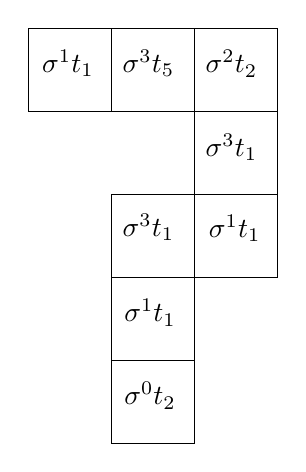
\begin{tikzpicture}[x=0.75pt,y=0.75pt,yscale=-1,xscale=1]
		%uncomment if require: \path (0,300); %set diagram left start at 0, and has height of 300
		
		%Shape: Square [id:dp721665415118685] 
		\draw   (320,230) -- (360,230) -- (360,270) -- (320,270) -- cycle ;
		%Shape: Square [id:dp32997086757969785] 
		\draw   (320,190) -- (360,190) -- (360,230) -- (320,230) -- cycle ;
		%Shape: Square [id:dp722013149285231] 
		\draw   (320,150) -- (360,150) -- (360,190) -- (320,190) -- cycle ;
		%Shape: Square [id:dp7194653668810835] 
		\draw   (360,150) -- (400,150) -- (400,190) -- (360,190) -- cycle ;
		%Shape: Square [id:dp5623142921410371] 
		\draw   (360,110) -- (400,110) -- (400,150) -- (360,150) -- cycle ;
		%Shape: Square [id:dp811276513166974] 
		\draw   (360,70) -- (400,70) -- (400,110) -- (360,110) -- cycle ;
		%Shape: Square [id:dp6460752823843325] 
		\draw   (320,70) -- (360,70) -- (360,110) -- (320,110) -- cycle ;
		%Shape: Square [id:dp09929285168542534] 
		\draw   (280,70) -- (320,70) -- (320,110) -- (280,110) -- cycle ;
		
		% Text Node
		\draw (325,239.4) node [anchor=north west][inner sep=0.75pt]    {$\sigma ^{0} t_{2}$};
		% Text Node
		\draw (325,199.4) node [anchor=north west][inner sep=0.75pt]    {$\sigma ^{1} t_{1}$};
		% Text Node
		\draw (324.2,158.2) node [anchor=north west][inner sep=0.75pt]    {$\sigma ^{3} t_{1}$};
		% Text Node
		\draw (365.8,158.6) node [anchor=north west][inner sep=0.75pt]    {$\sigma ^{1} t_{1}$};
		% Text Node
		\draw (364.2,119.8) node [anchor=north west][inner sep=0.75pt]    {$\sigma ^{3} t_{1}$};
		% Text Node
		\draw (364.2,79.4) node [anchor=north west][inner sep=0.75pt]    {$\sigma ^{2} t_{2}$};
		% Text Node
		\draw (324.2,79) node [anchor=north west][inner sep=0.75pt]    {$\sigma ^{3} t_{5}$};
		% Text Node
		\draw (285.4,79) node [anchor=north west][inner sep=0.75pt]    {$\sigma ^{1} t_{1}$};
		
		
	\end{tikzpicture}
\end{figure}
 	
	
	
	\section{Discussion}
	The formulation above is very promising for me. One possible reason for this is the following observation:
	\begin{observation}
		Any valid tiling corresponds the branching annihilating random walks on the graph $ A = A_v \oplus A_h $, where $ \oplus $ operation adds a bidirectional edge between two nodes with the same name on $ A_v $ and $ A_h $.
	\end{observation}
	So it opens up lots of useful results form stochastic processes and and probability theory. Furthermore, seeing these graphs as the state space of some Markov chain and the long term properties of this chain can have real world implications of the possible assemblies. 
	
	Furthermore, one can add different weights to the edges, corresponding to the strength of the corresponding glue-glue interaction. Then certain path's on the graph will be more probable than the other ones, and using the observation above, regarding the correspondence between branching-annihilating walks on $ A $ and valid tile assemblies, this translates to higher possibility of observing certain assemblies compared to other ones.
	
	Also, the graph $ A $ if very similar to the state space of a Turing machine, and I am also curious to see what will be the tiling implications of certain finite automate designs, like the ones that can detect certain string patterns etc.
	
	Furthermore, encoding all the valid tilings in $ A $, then one can design ``smart'' tiles. For instance, the tiles that are dead end and once a random walker gets there can not get out. This kind of tile would correspond to the ``capping'' tiles that stop the growth in certain direction.
	
	Furthermore, it is very straightforward to extend this formulation for cubic tiles in 3D, or other tiles like hexagonal tiles in 2D. For instance, in the case of $ 3D $ cubes, if we allow rotation, then we would have two rotation operators $ \sigma $ and $ \tau $, and we will consider different powers of these operators from 0 to 3. In the case of hexagonal lattice, we will still have one rotation $ \sigma $, which is 60 degrees counterclockwise rotation, and we will have the powers $ 0 $ to $ 5 $ of this operator. So different tiling grids and different dimensions will only translate to richer rotation operators.  
	
	
	
\end{document}